\documentclass{article}
\usepackage{parskip}
\usepackage{pdfpages}
\usepackage[margin=.6in]{geometry}
\begin{document}
Somehow I missed a bunch of stuff, sorry future lara.
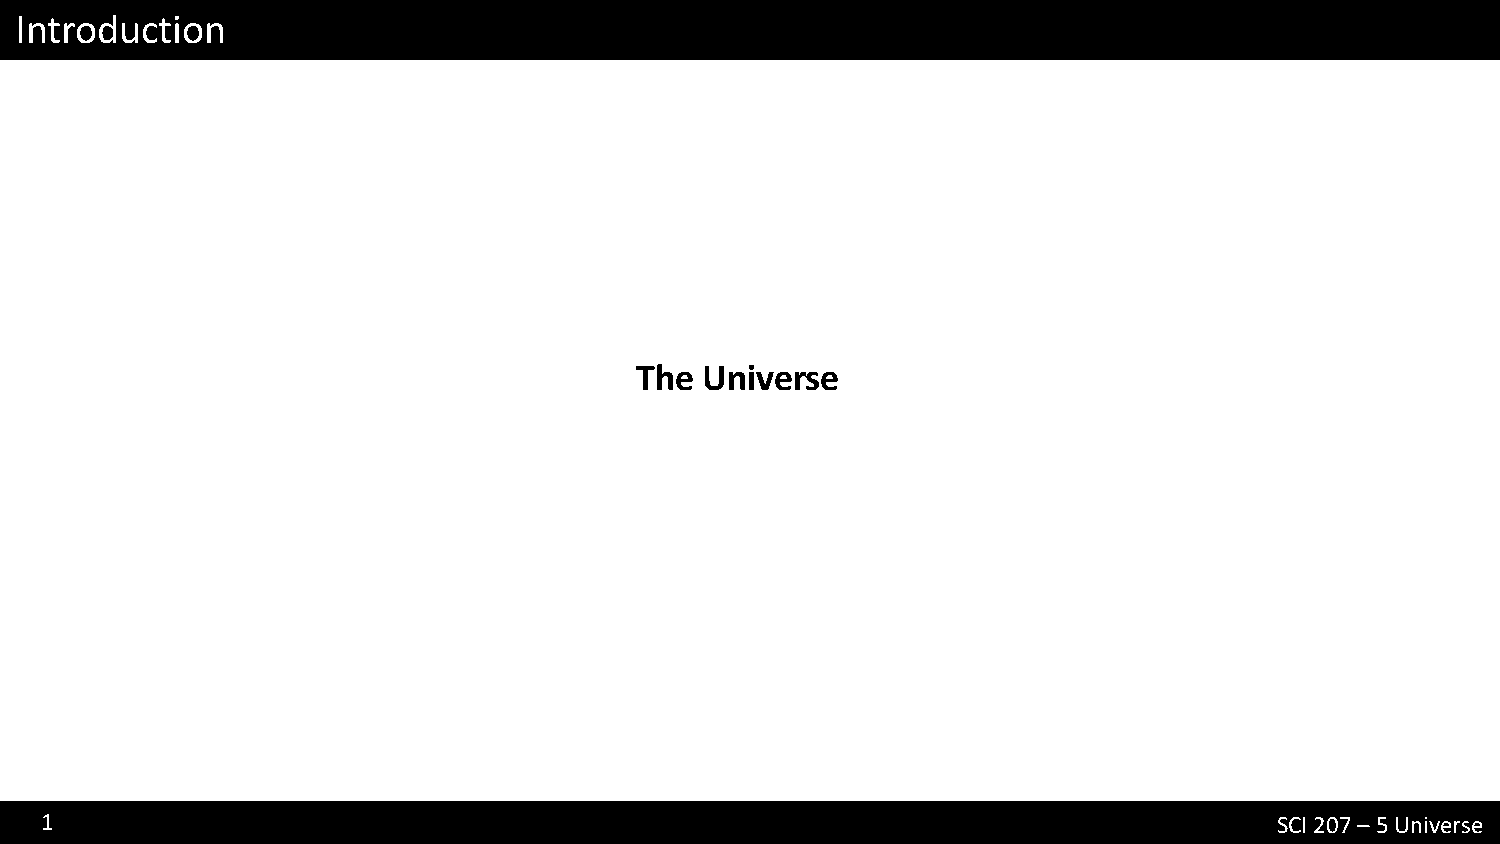
\includepdf[page=1-39]{slides}
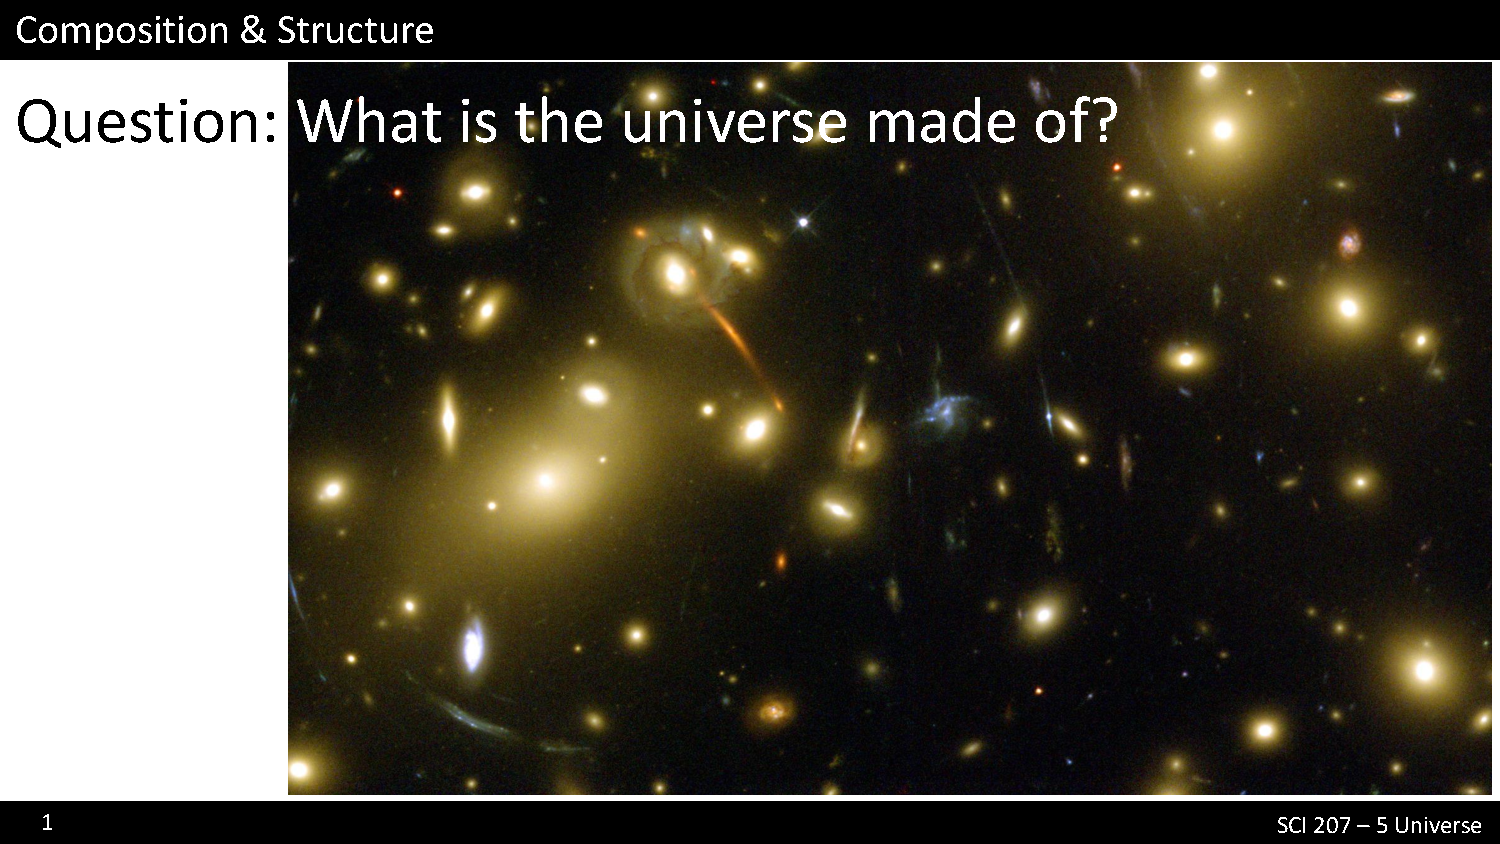
\includepdf[page=1-5]{slides2}
Basically after tons of years we found that the universe is made up of basically stars, gas, and dust. Mostly Hydrogen, Helium, and small amounts of heavier elements.

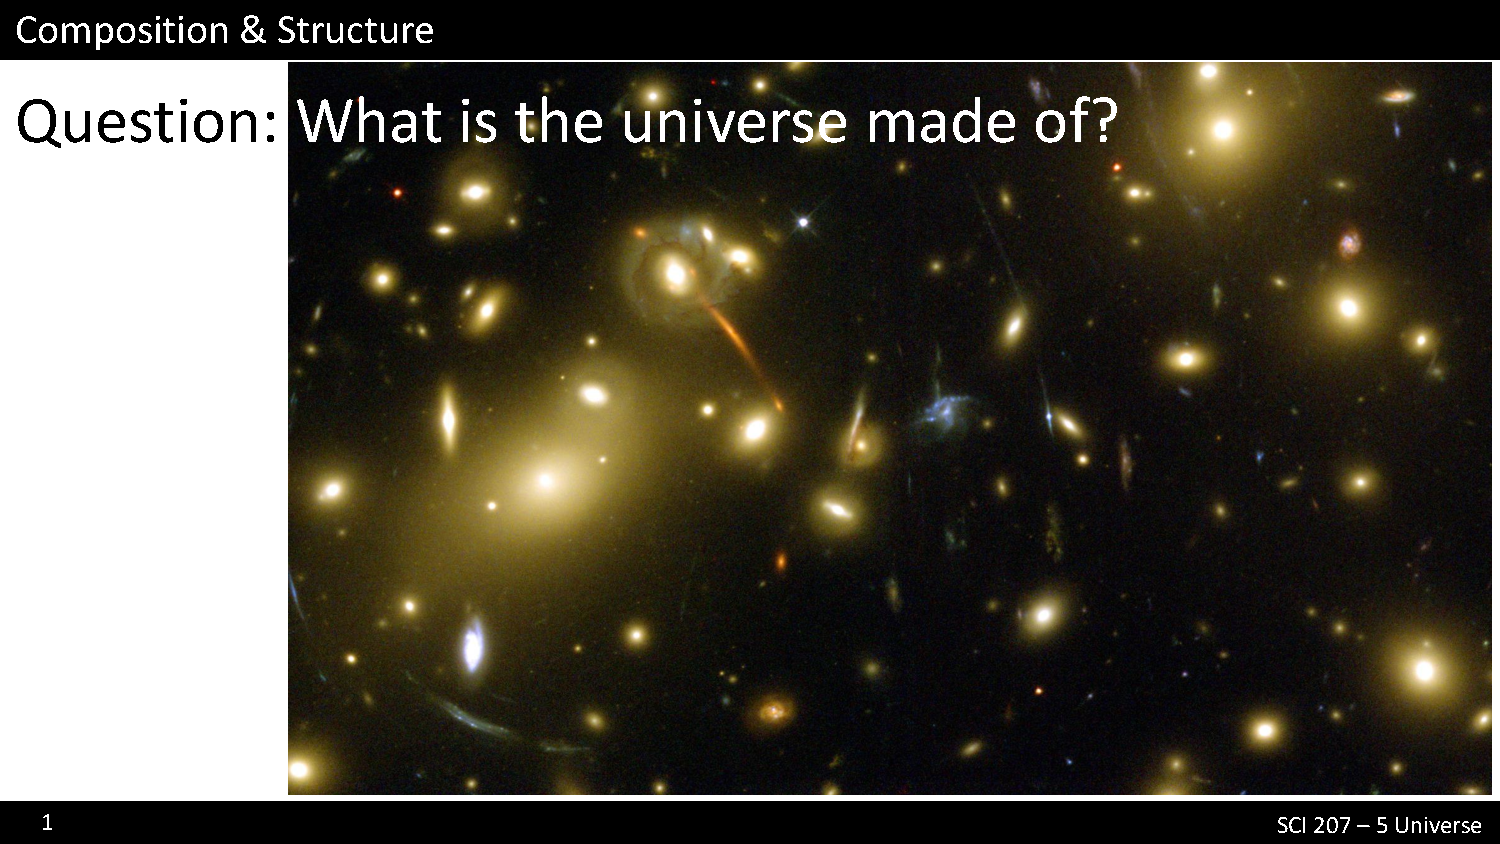
\includepdf[page=6]{slides2}
When looking at the stars we saw a bunch of distortions that couldnt actually represent something real. These we know are caused by gravity.

Basically everything is mass-energy. It is all mass that has inertia. All that mass out there warps space-time. As light moves from a region of slow time to a region of fast time light gets red shifted. This happens around massive objects.

Massive objects also have extra space around them, best visualized by the warping of a fabric with a weight on it. This is how gravity bends light

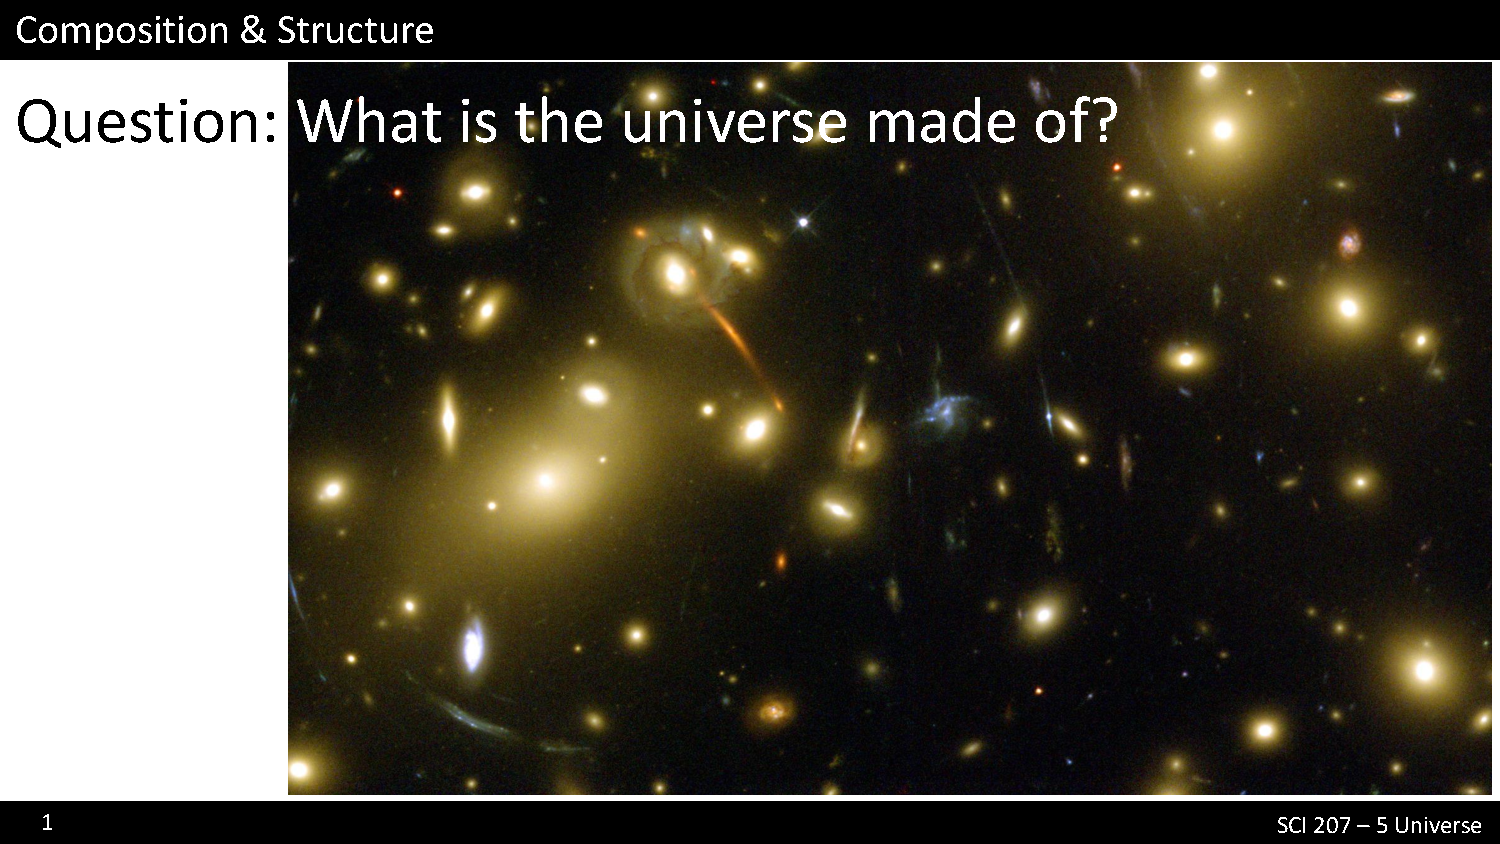
\includepdf[page=7]{slides2}
Light always moves at the same speed. Mass warps time so that time moves more slowly near the mass. Time warping tilts the wave fronts near mass, this causes the array of light to bend around the mass.

Mass also warps space around it. There is more space for the light to go through.

Note: light always travels in a striaght line, its the space-time through which is travels that is bent.

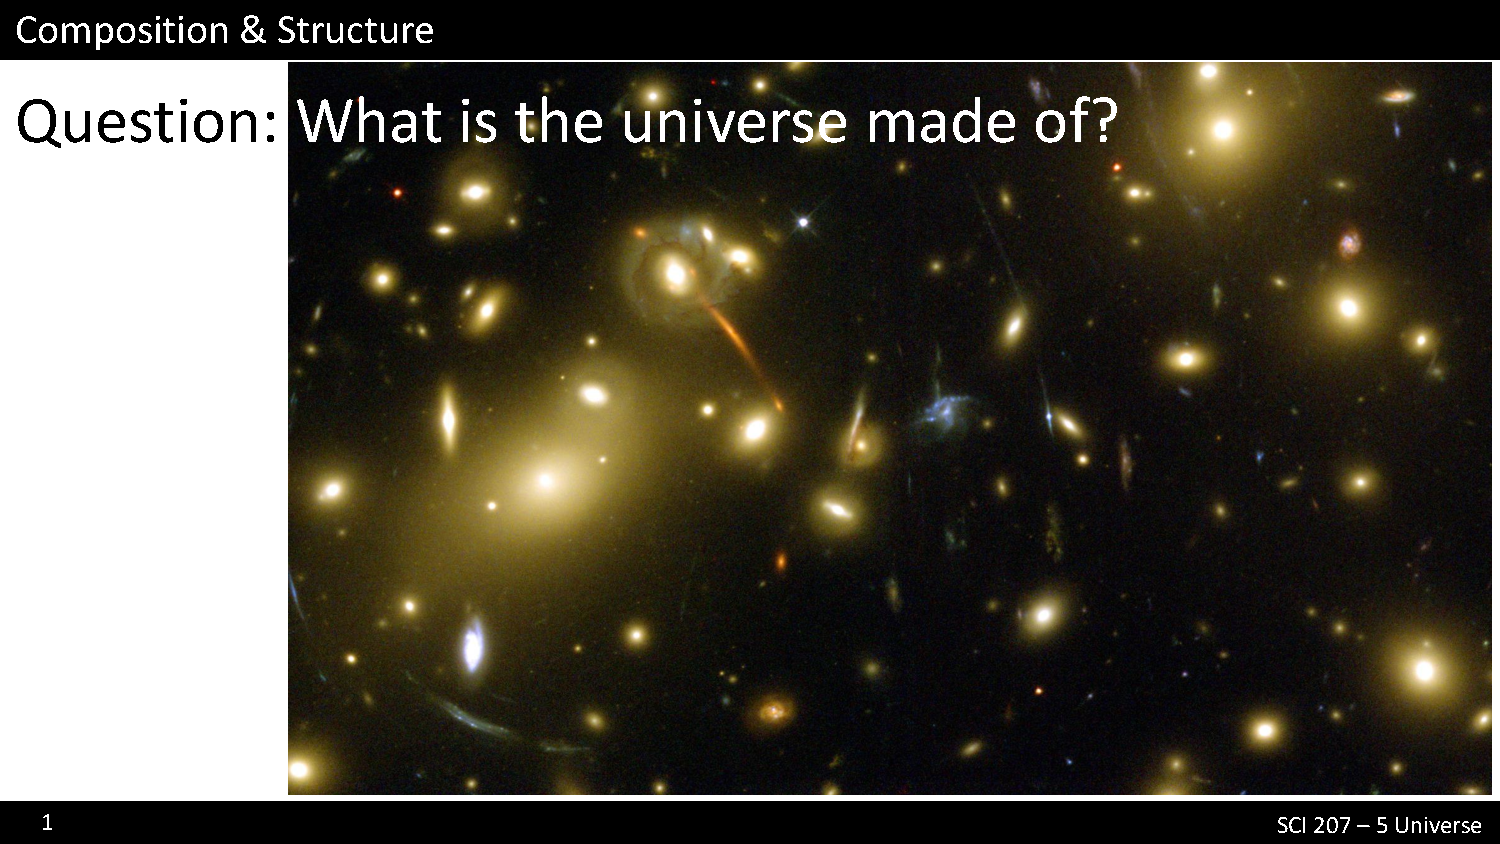
\includepdf[page=8]{slides2}
This image shows how we can view things behind the sun.

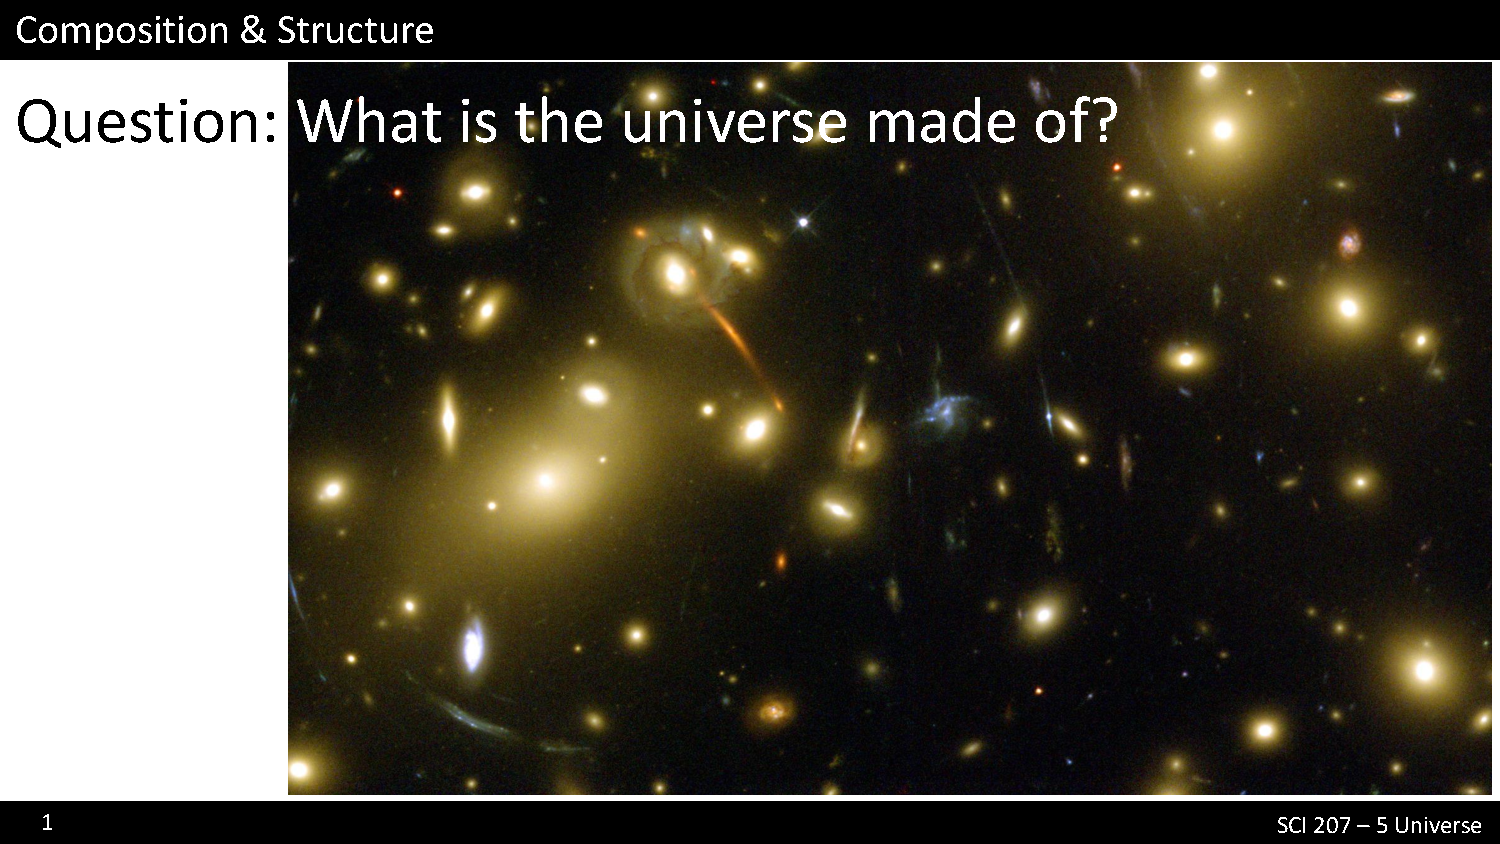
\includepdf[page=9]{slides2}
Any amount of mass-energy will create this lense of bent light. This lets us known that all mass can be ``seen'' regardless of whether visible light can be bounced off it.

We can see here how the bending of light will cause \emph{Einstein rings}.

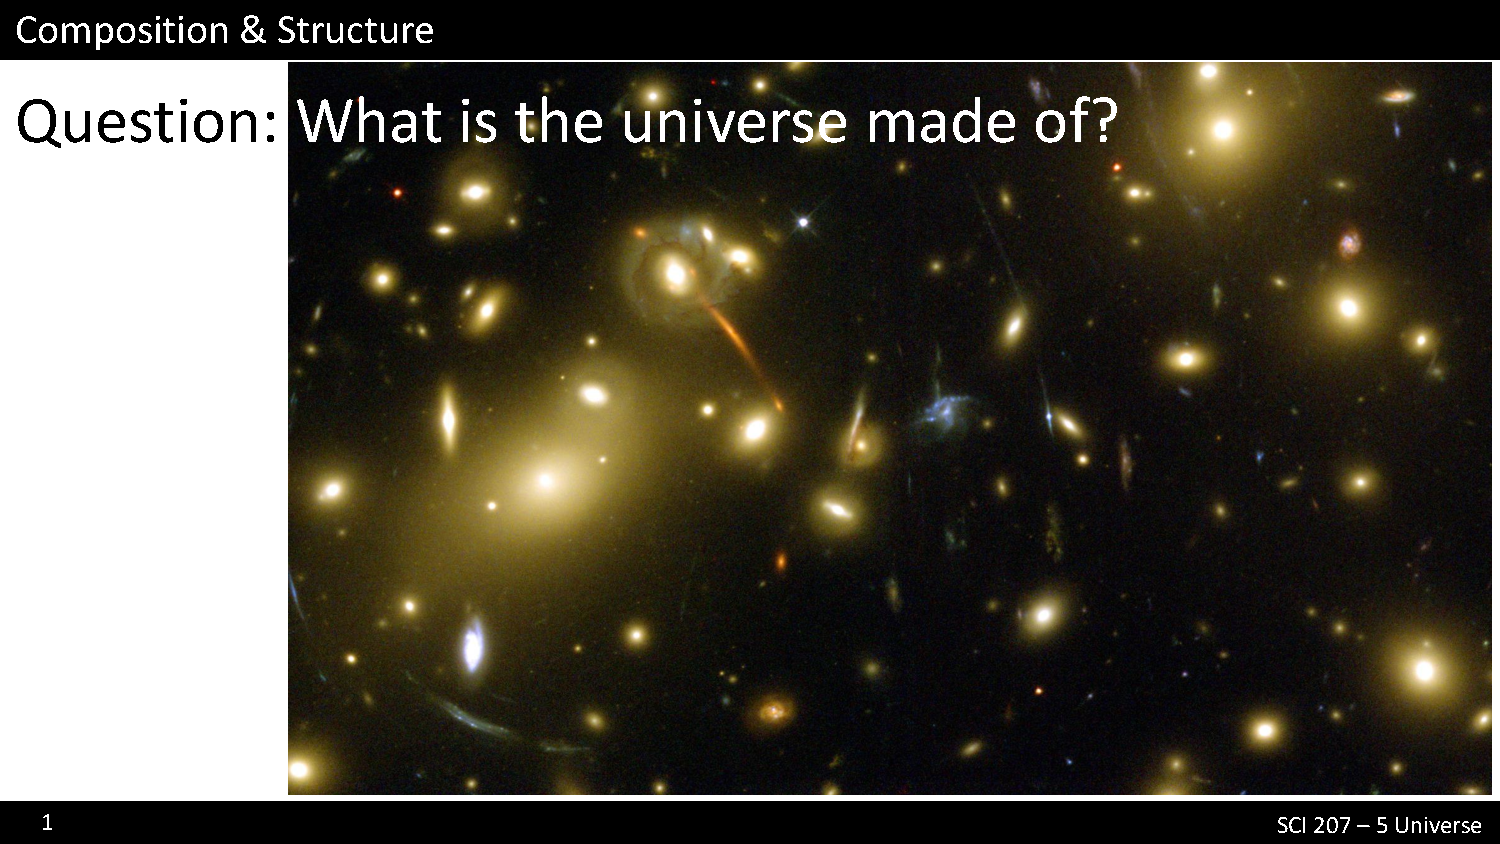
\includepdf[page=10-12]{slides2}
We can use the light distortions we see to create a 3D image of all the mass in the galaxy.

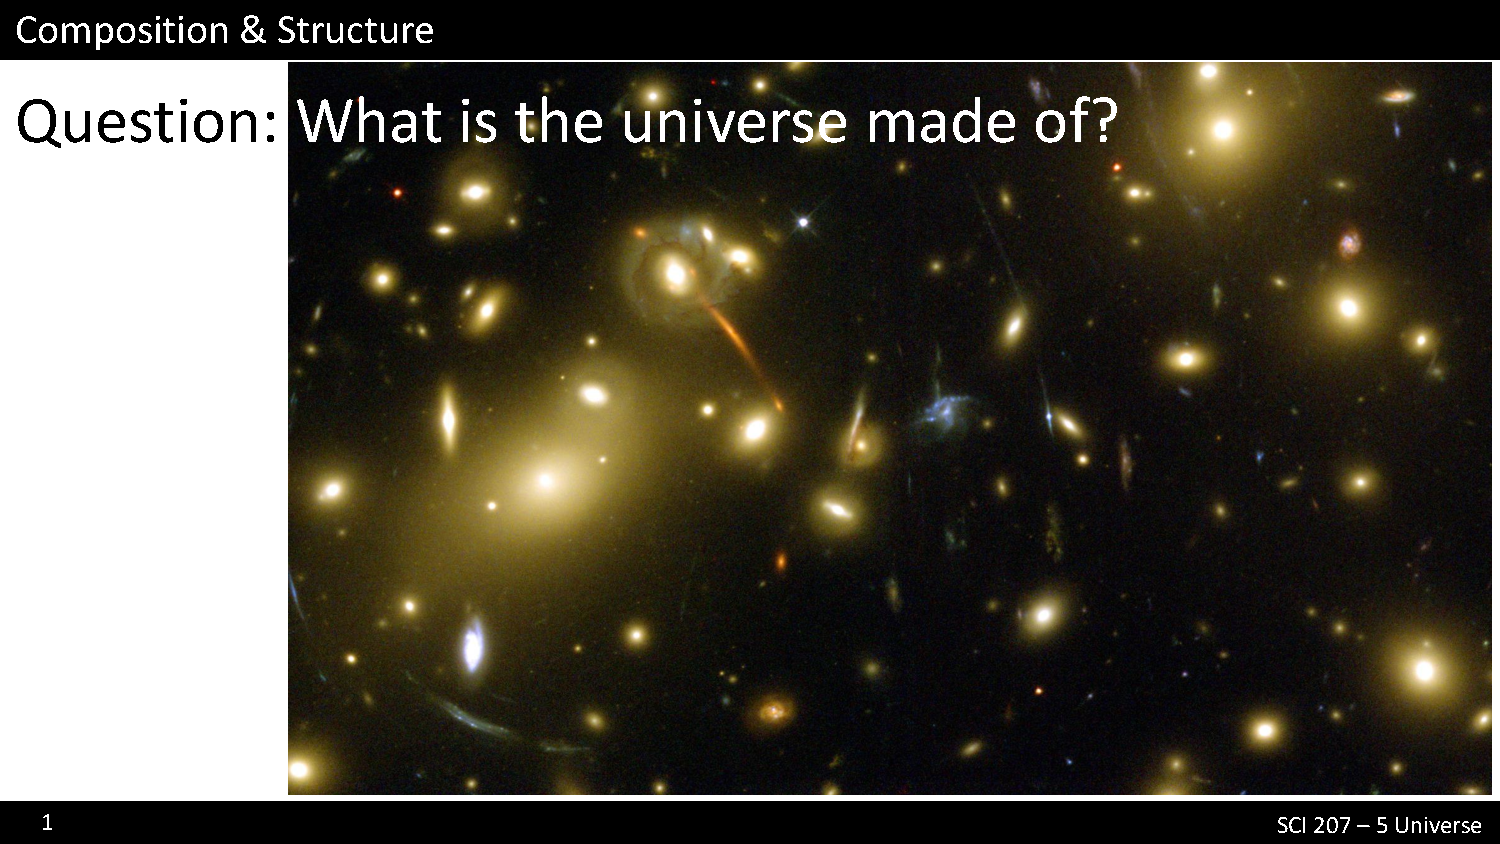
\includepdf[page=13]{slides2}
The results of our research into the mass of the universe has revealed that 85\% of all mass is dark.

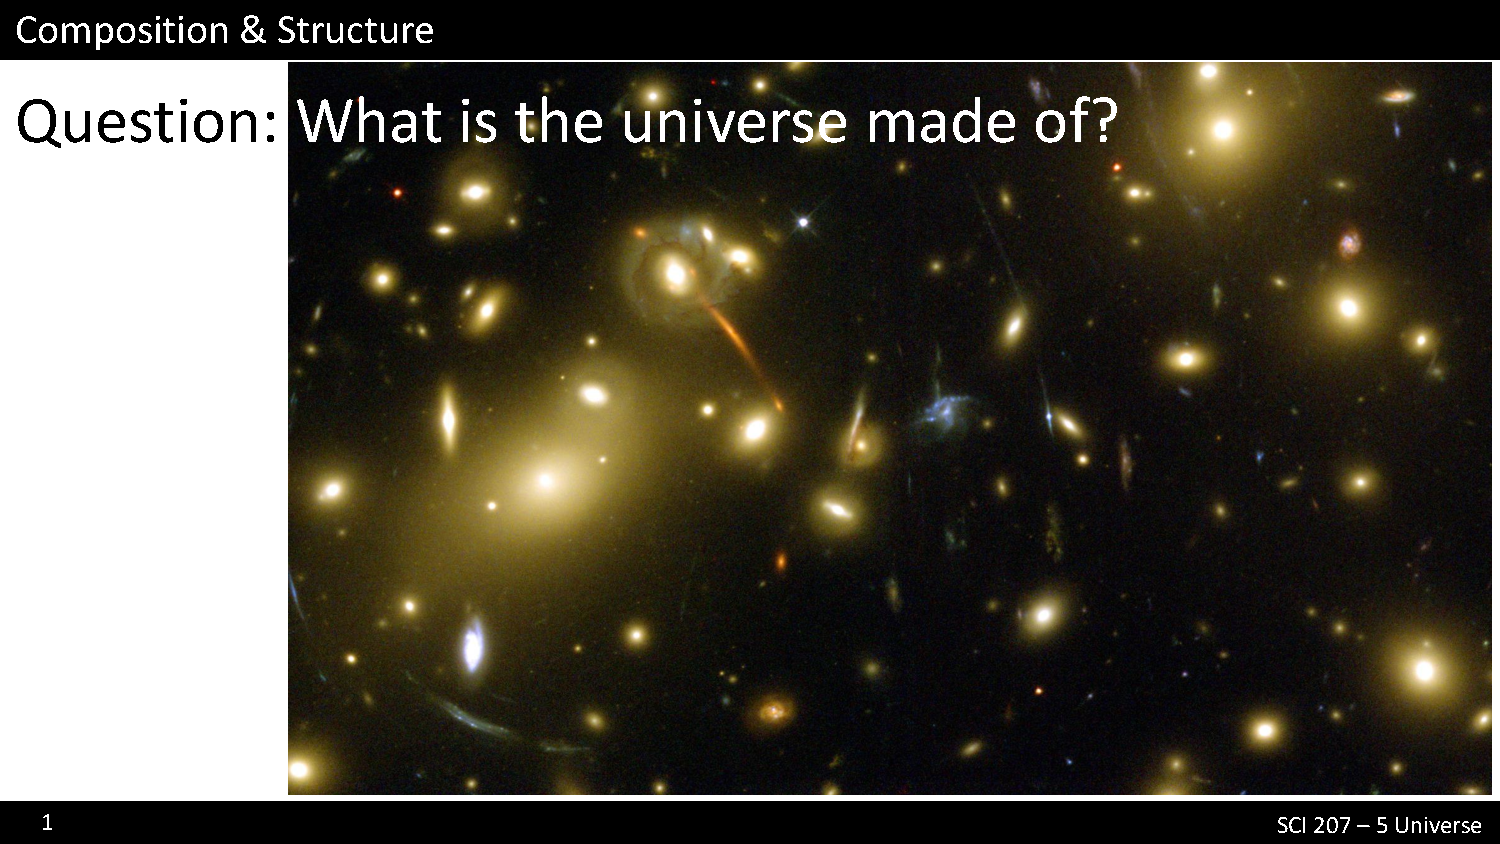
\includepdf[page=14]{slides2}
This picture shows what it would be like if we could see dark matter.

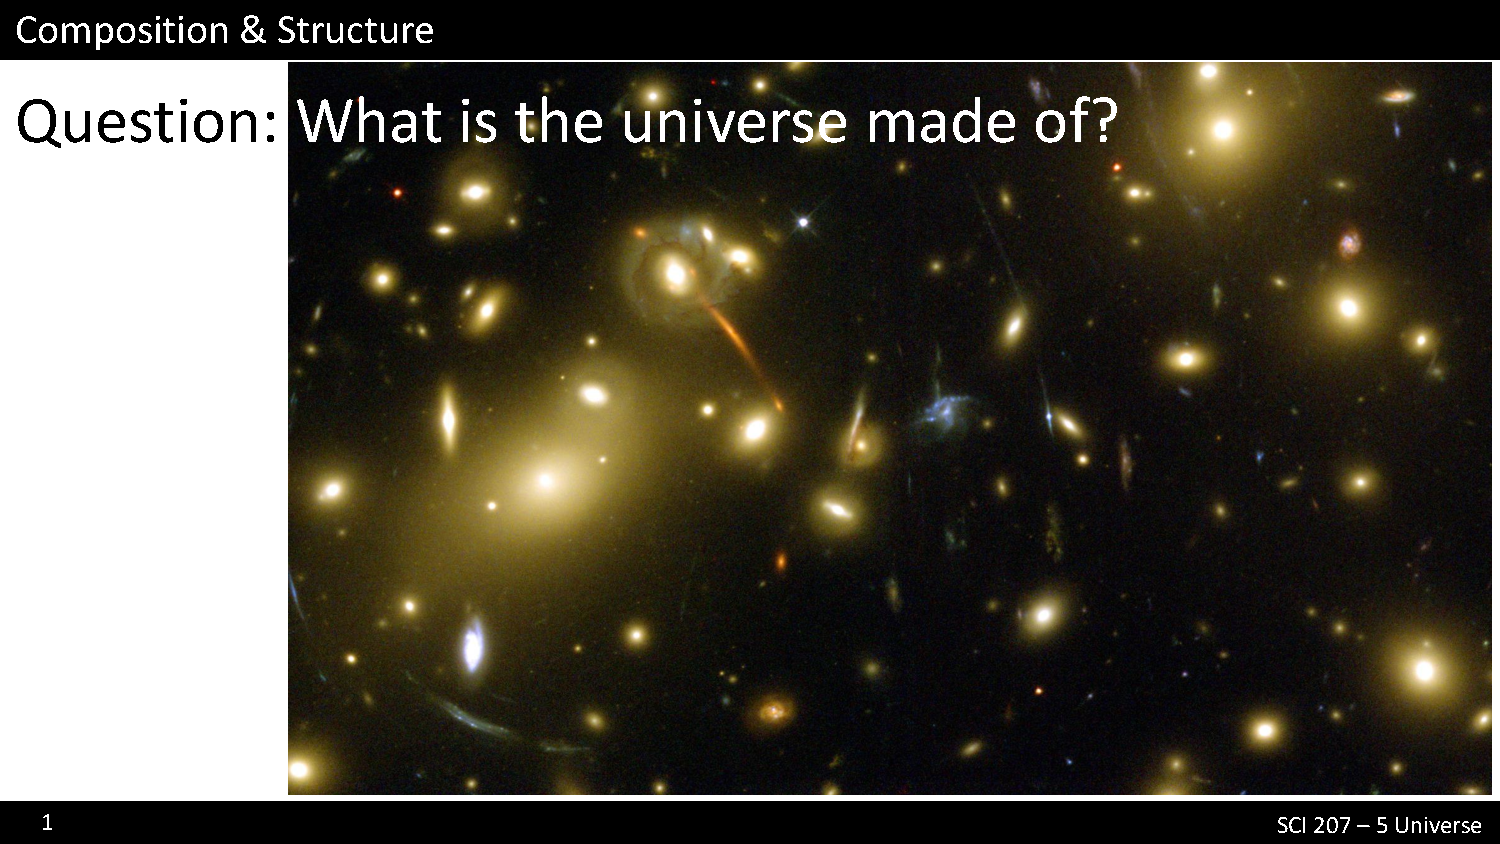
\includepdf[page=15-16]{slides2}
The claim that dark matter eixsts requires a lot of evidence to back it up. There are 5 different proofs. Gravitational lensing is one.

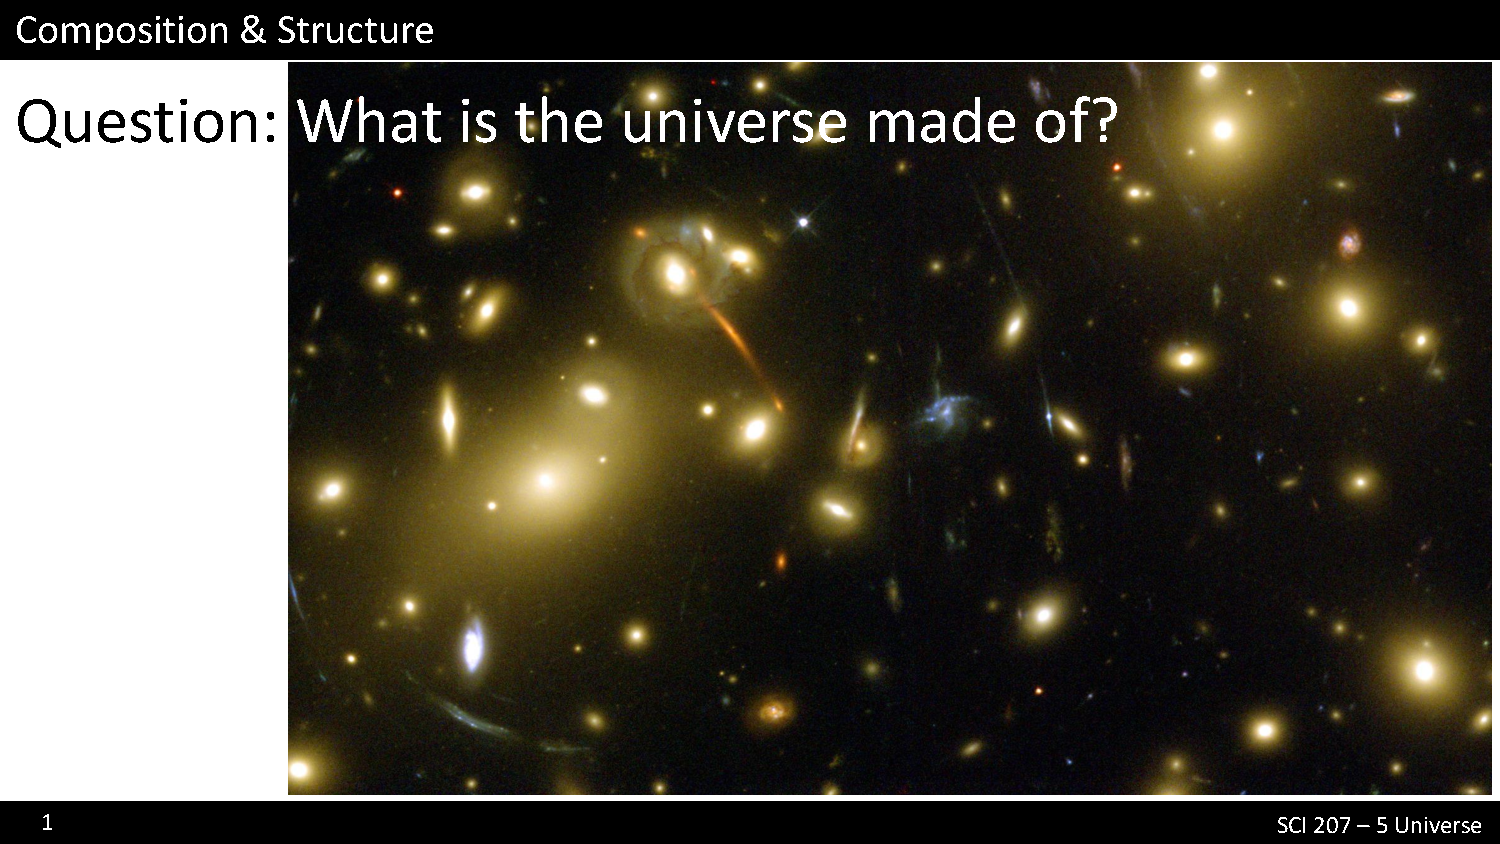
\includepdf[page=17]{slides2}
Galaxy rotation curves are another proof of the existence of dark matter.

We expect that since most of the mass of the galaxy is in the center, the stars on the edges are like planets orbiting the center. This means that their orbiting speeds should slow as we get farther from the center.

Vira Rubin looked at galaxy rotation and found that the speeds on the edges of the galaxy are basically the same. This would be caused either by gravity working weirdly, or a bunch of extra mass involved.

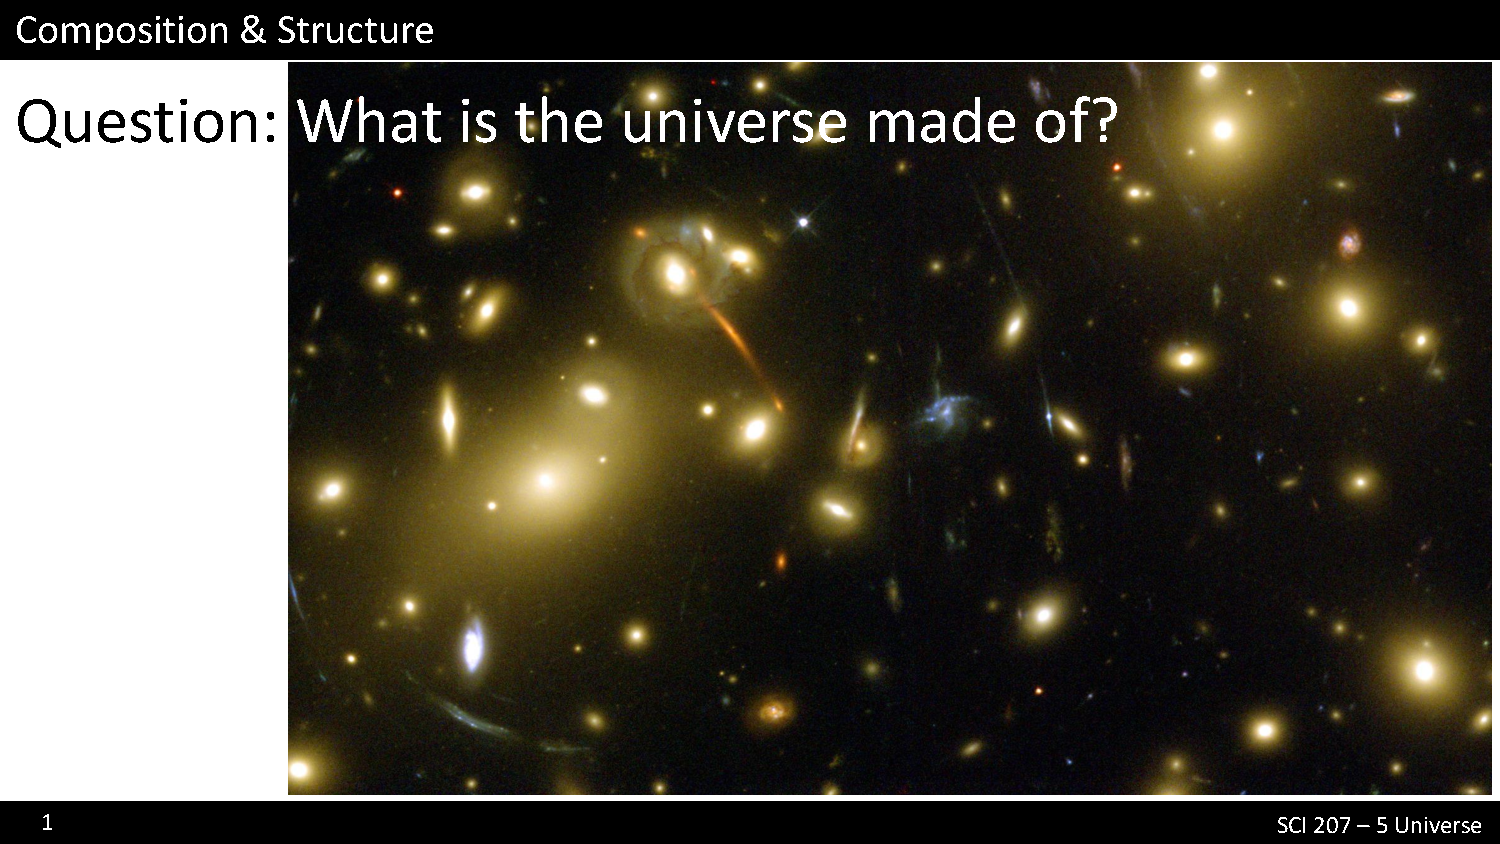
\includepdf[page=18-20]{slides2}
When galaxies collide very few starts actually collide due to how small they are relative to the size of the space between them.

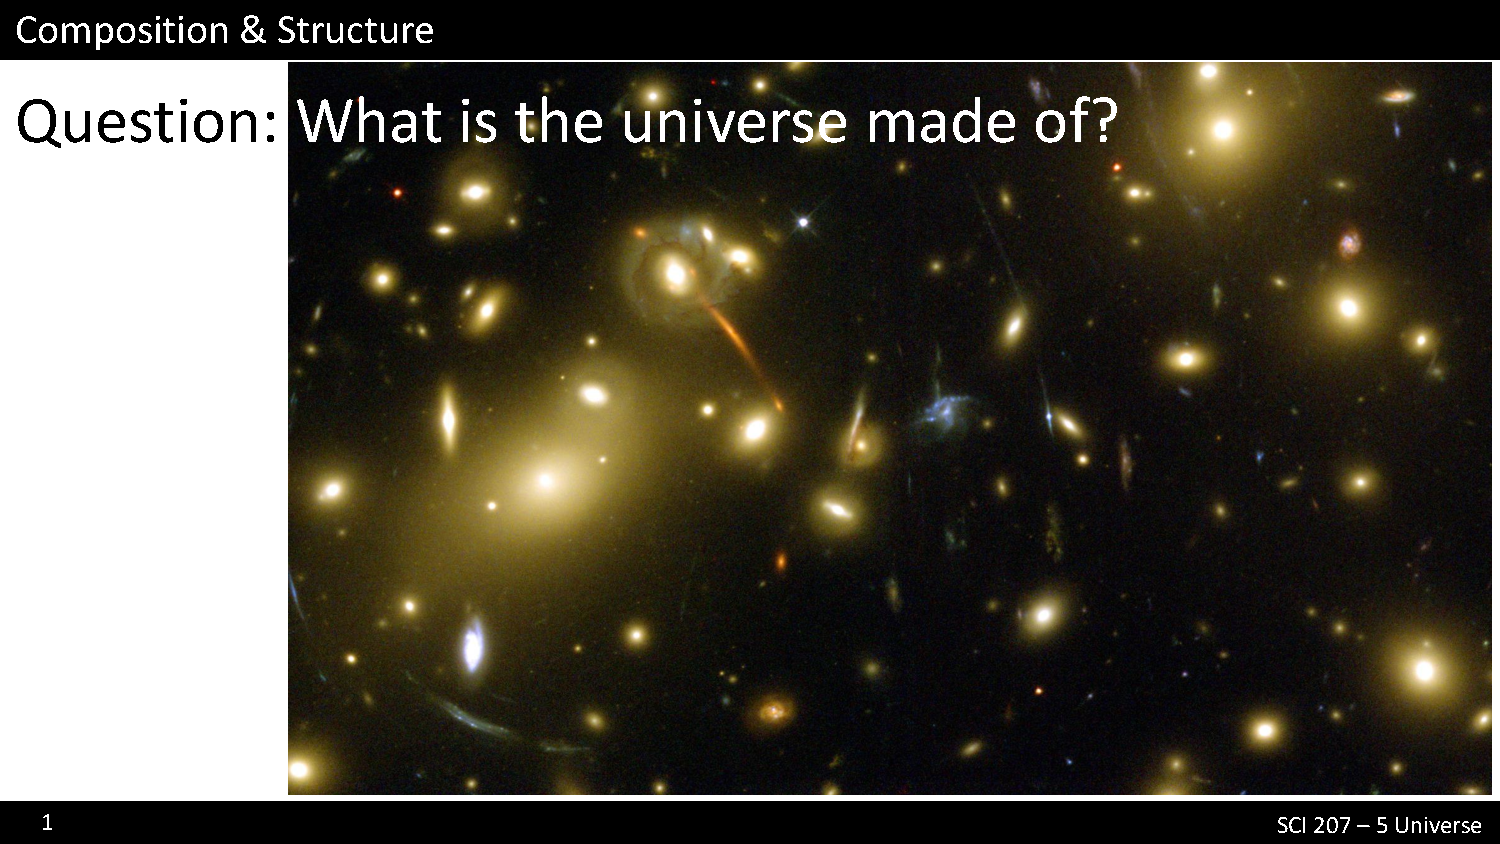
\includepdf[page=21]{slides2}
The big bang is not, there was nothing and then something exploded. The big bang is that the space is uniformly filled with matter and radiation so as we go back in time all that shit must have occupied a very small volume.

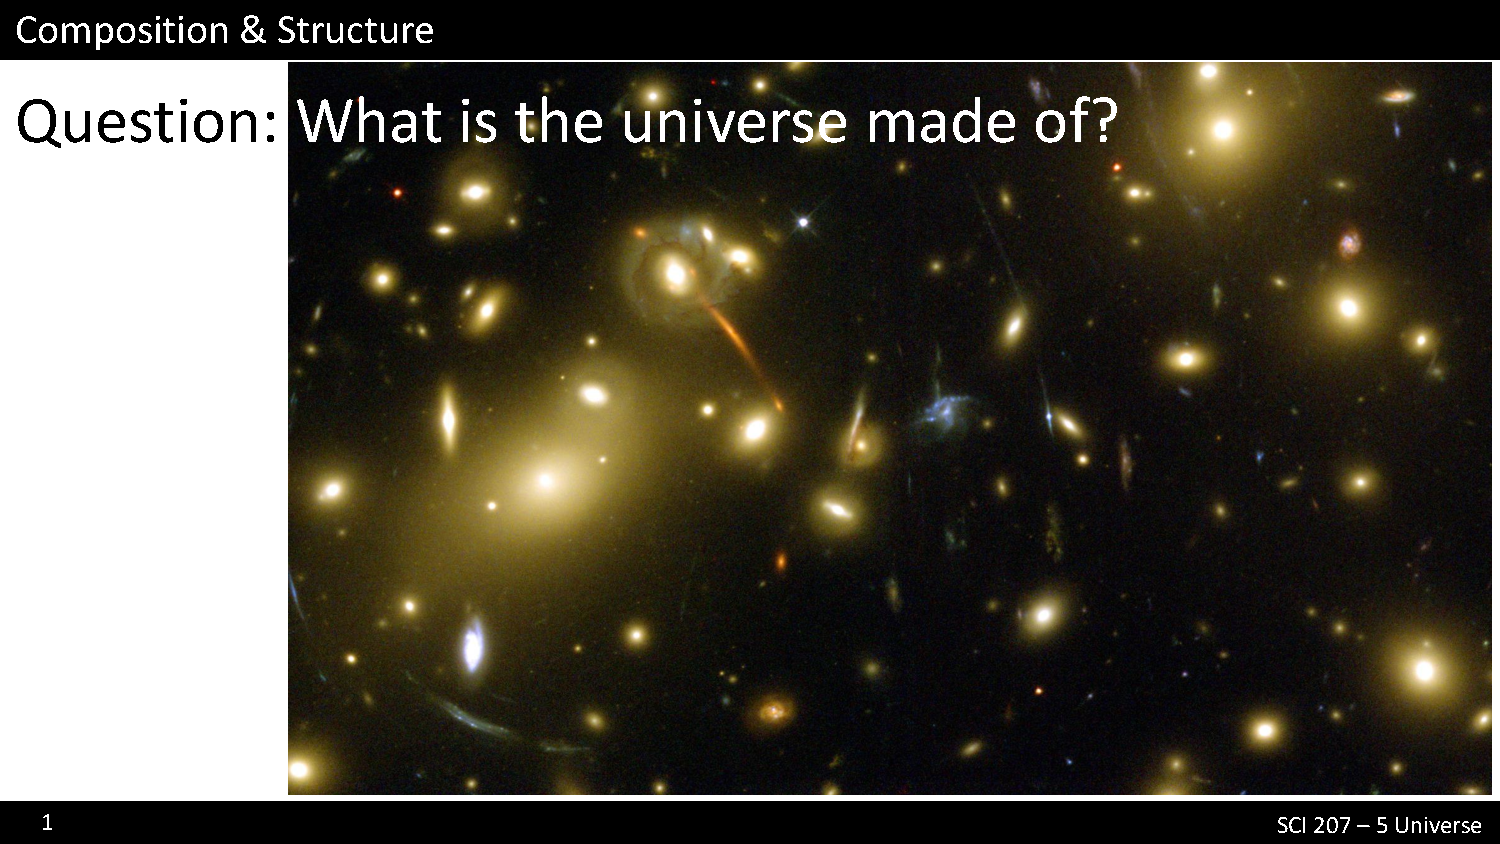
\includepdf[page=22]{slides2} next
Along the axis here is the milky way galaxy (this is just the universe close to us).


``The first time, that he came to me I was a young boy little did I not believe, there was a hole in my heart and I was looking for a piece that fit.''
-Notes by Steven

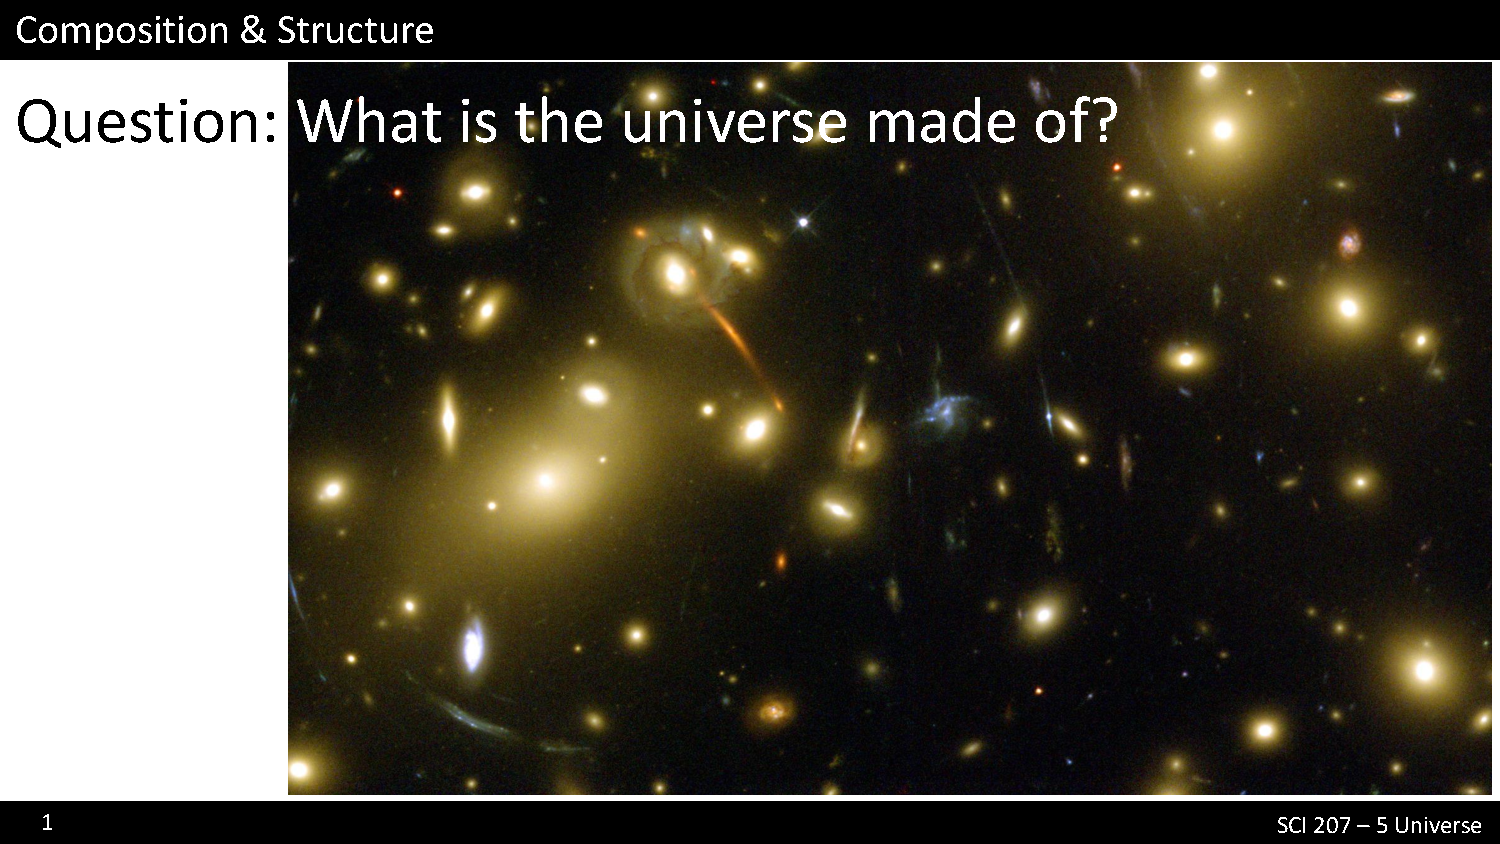
\includepdf[page=23-24]{slides2}
Baryonic means that its matter made up of protons and neutrons (so regular matter is this). Nucleo synthesis was a time at the start of big bang where protons and neutrons were very hot and slamming into eachother, causing fusion.

About one fifth of the atoms in the universe are involved in a process that makes them visible. Black holes are an example of ordinary matter that is dark.

Most of the dark matter must be non-baryonic.

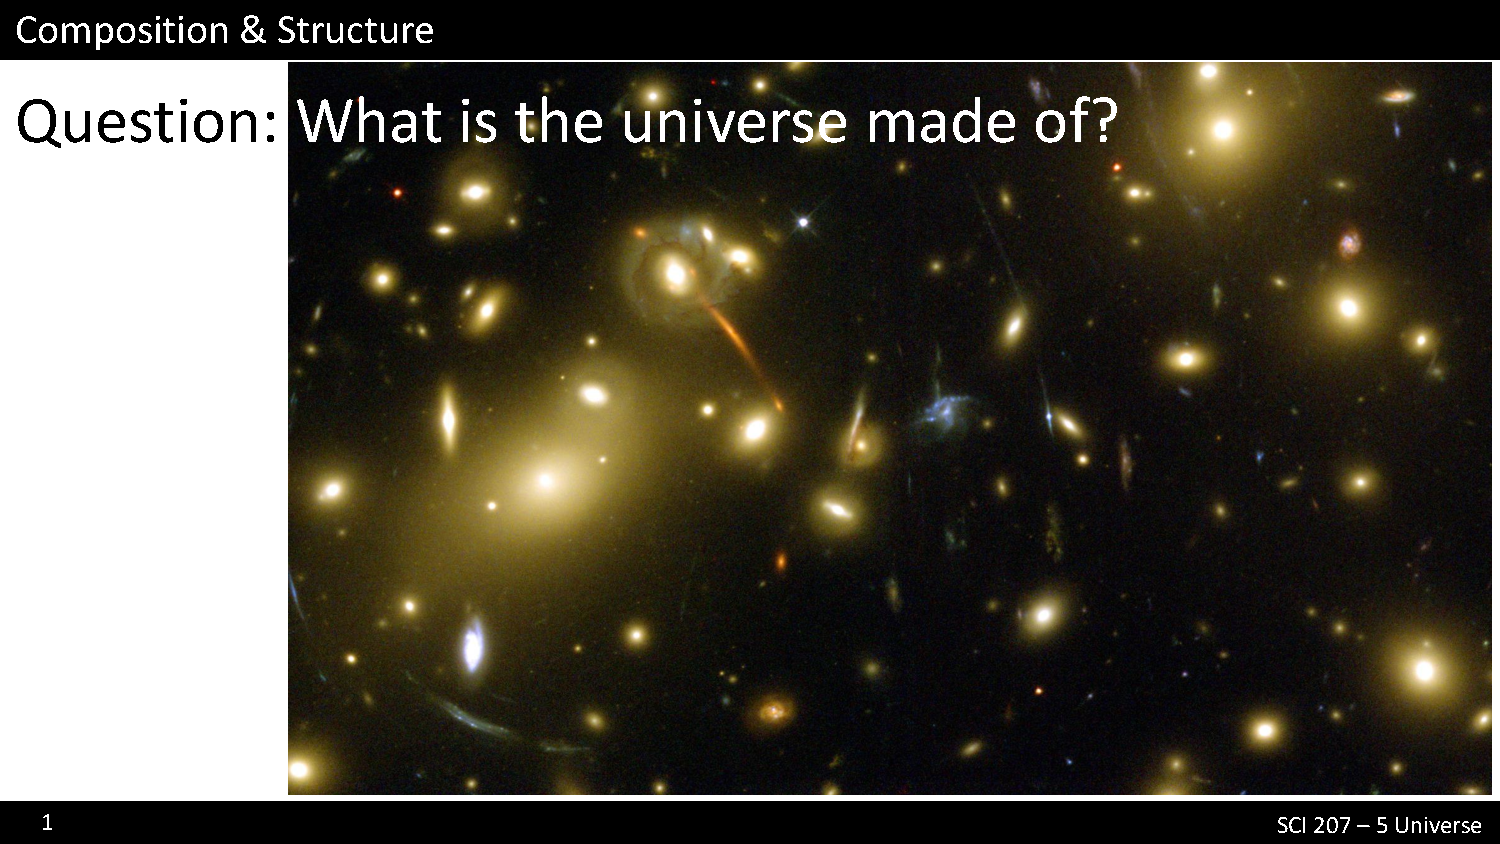
\includepdf[page=25]{slides2}
Dark matter could be hot or cold. Hot dark matter would be something like neutrinos (they are the second most abundant particle, after photons). They are very hard for us to catch. For every proton of ordinary matter there are a billion neutrinos. They are produced at the center of the sun. The react very poorly with matter so they pass through it very easily without being effected.

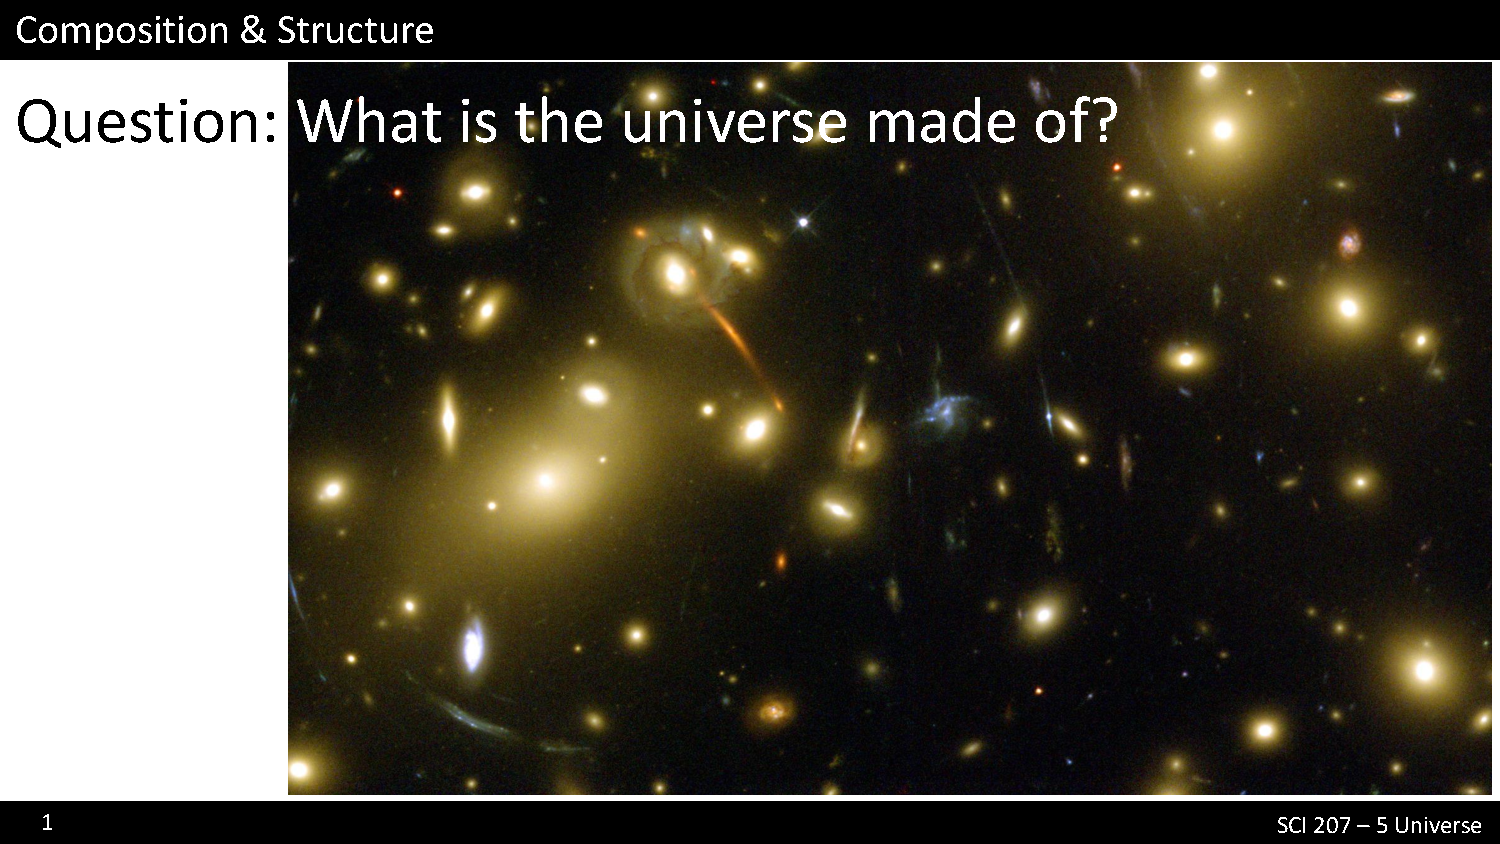
\includepdf[page=26-29]{slides2}
We've basically rulled out the theory that we need a modified view of gravity is wrong using the bullet cluster theory.

Some people are looking at more dimensions as an issue. This leads to super string theory.

There were defects in the quantum field that caused energy, and thus gravity which could have lead to some of the dark matter we can't see.

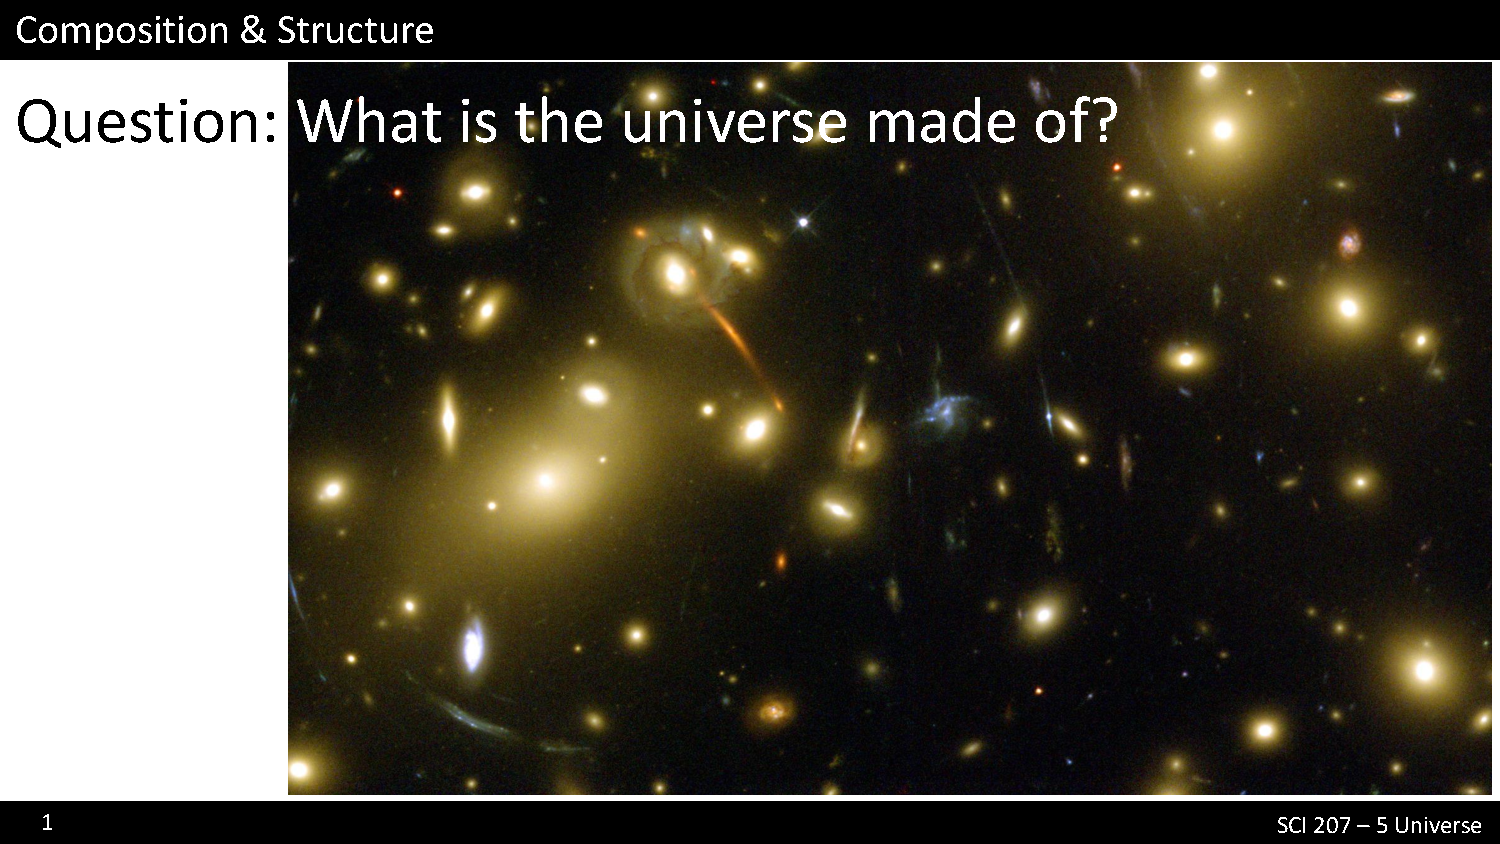
\includepdf[page=30-36]{slides2}

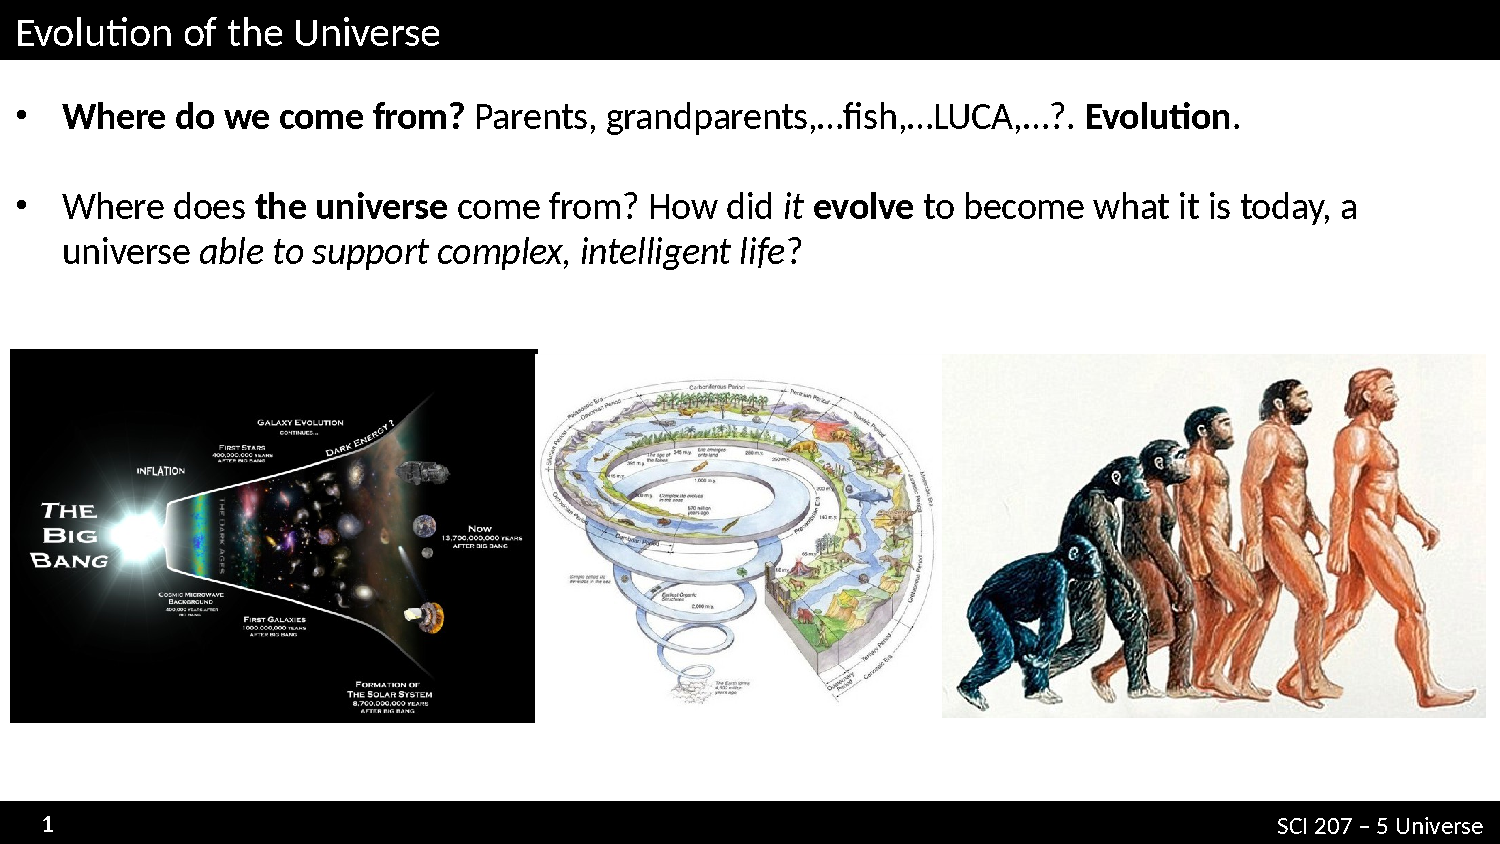
\includepdf[page=1-2]{slides3}
Einstein thought of a universe that was finite in size but without boundaries (think of a sphere, you cannot fly off the edge). He knew that the universe must be dynamic so either expanding or contracting. To test it he introduced a constant called the cosmological constant to his equations which simplified them greatly.

%this is slide 80 in the full set
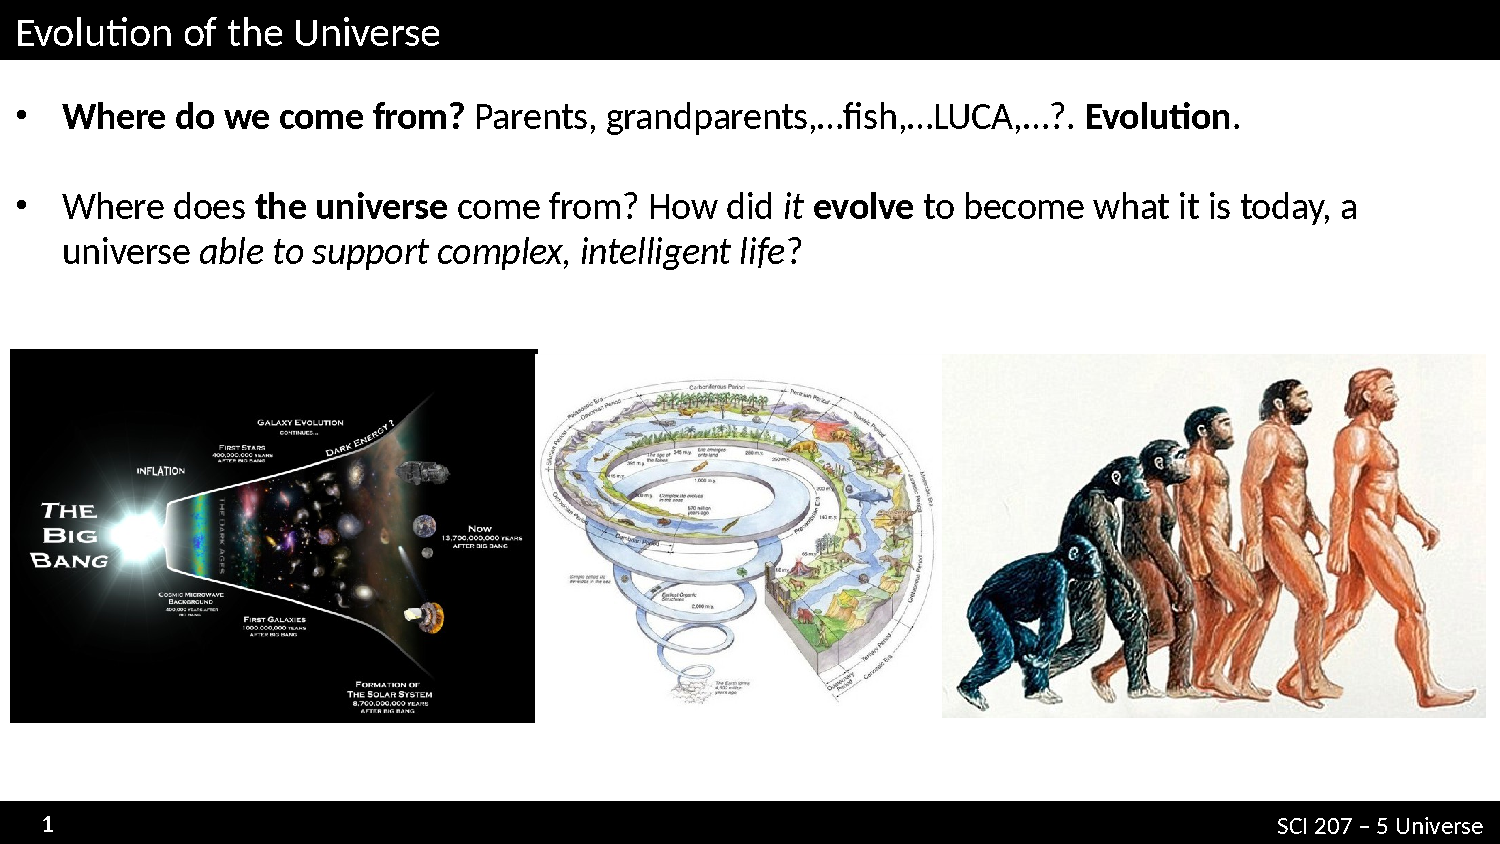
\includepdf[page=3]{slides3}
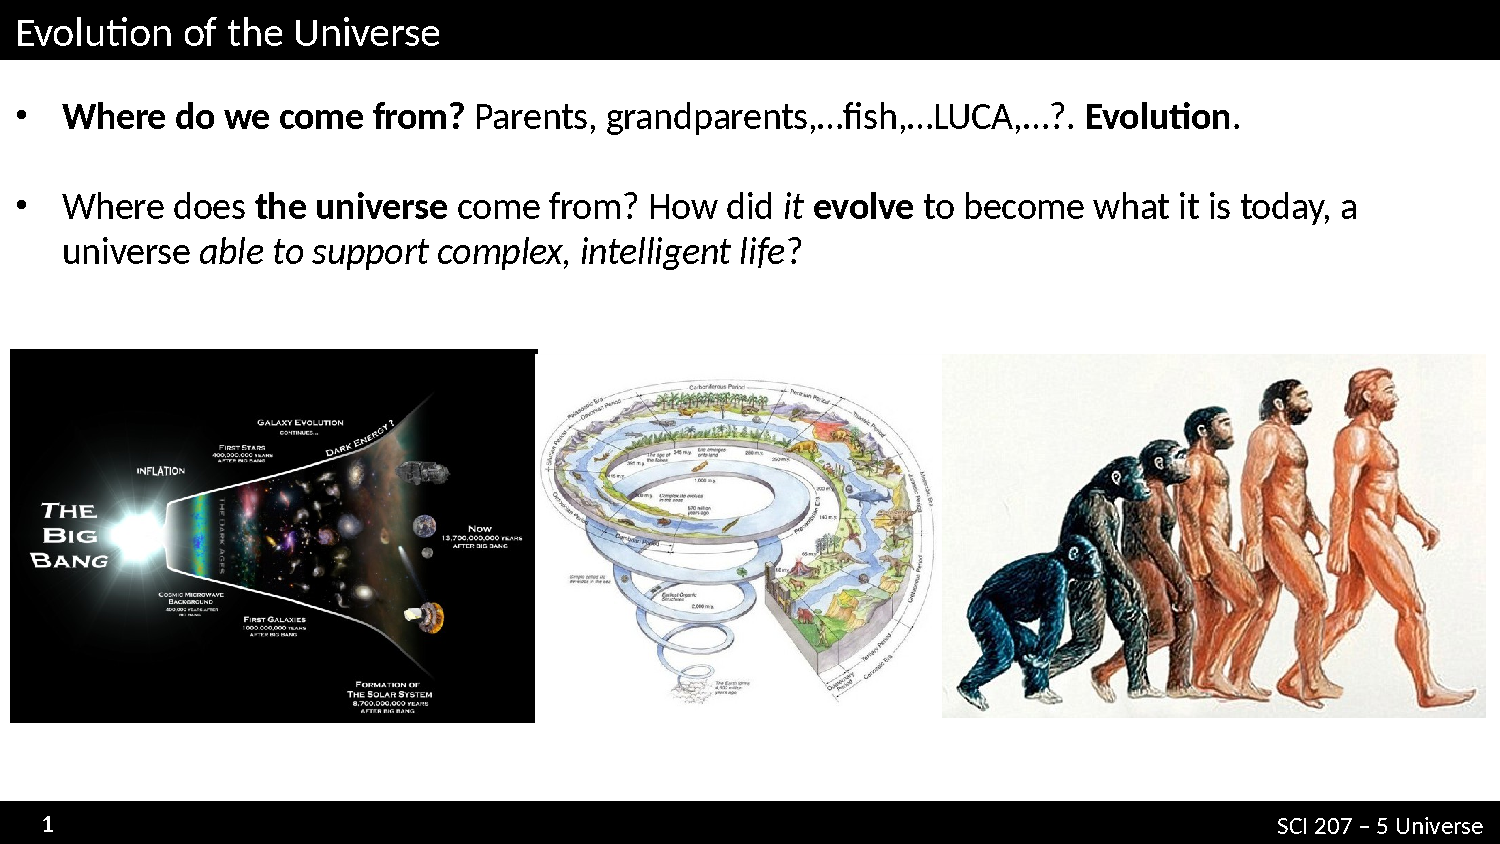
\includepdf[page=4]{slides3}
Friedman realized that if you assume that the universe is uniformly distributed then einsteins theroy tells you there are 3 forms of space.
\begin{itemize}
	\item infinite in size and flat
	\item infinite in size and curved
	\item finite and spherical
\end{itemize}
He used the notion of 3 galaxies and if you drew lines of light between them to explain these options

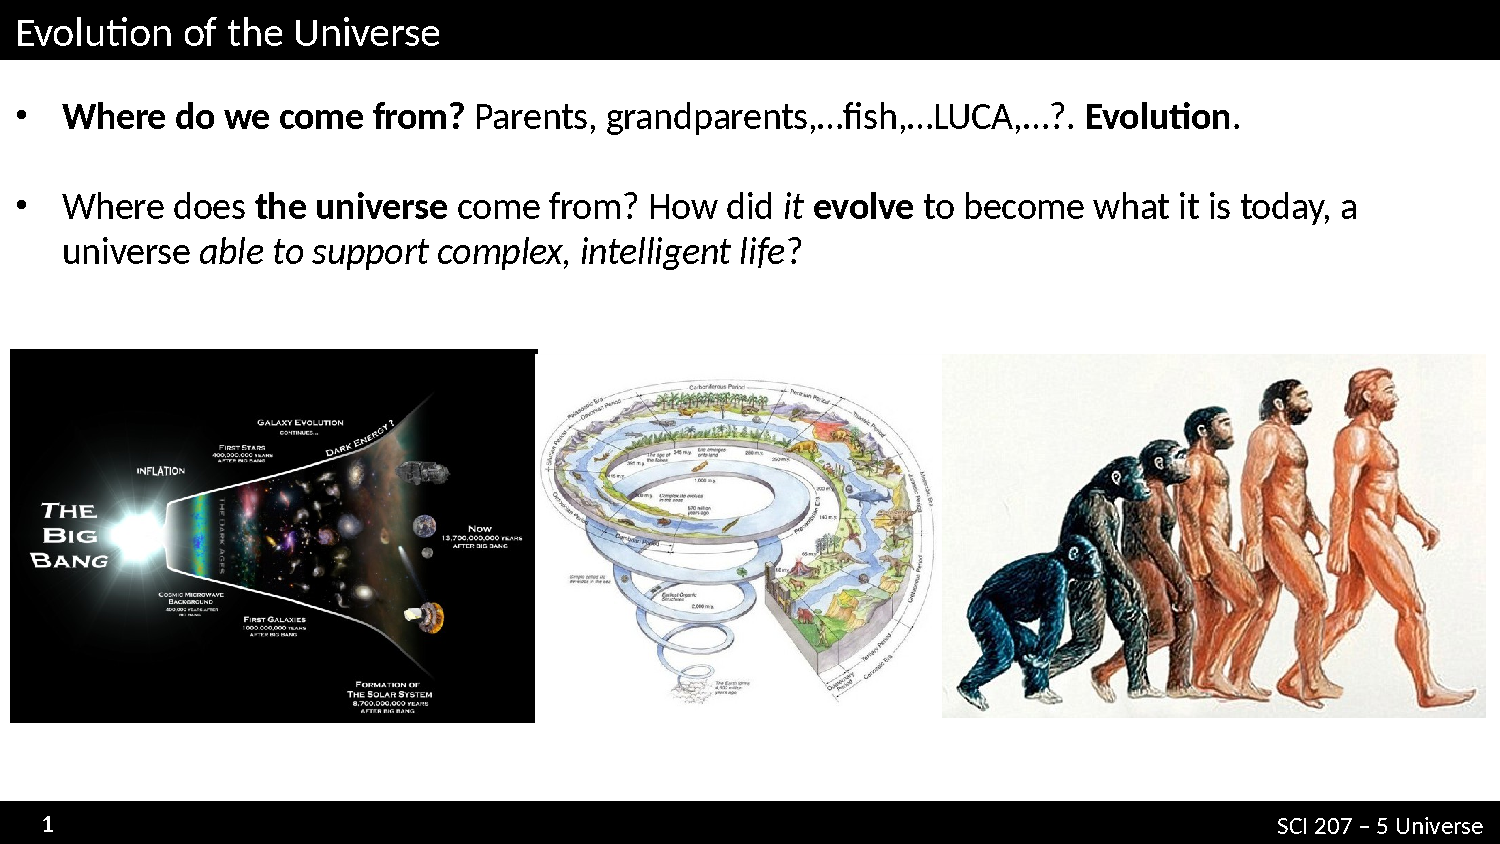
\includepdf[page=5]{slides3}
If the universe is dynamic it had to have a start and an end. Lemaitre came to the same conclusions and Friedman and also knew about red shifts. From this he derives that the universe started with an explosion. He called this the primeval atom.
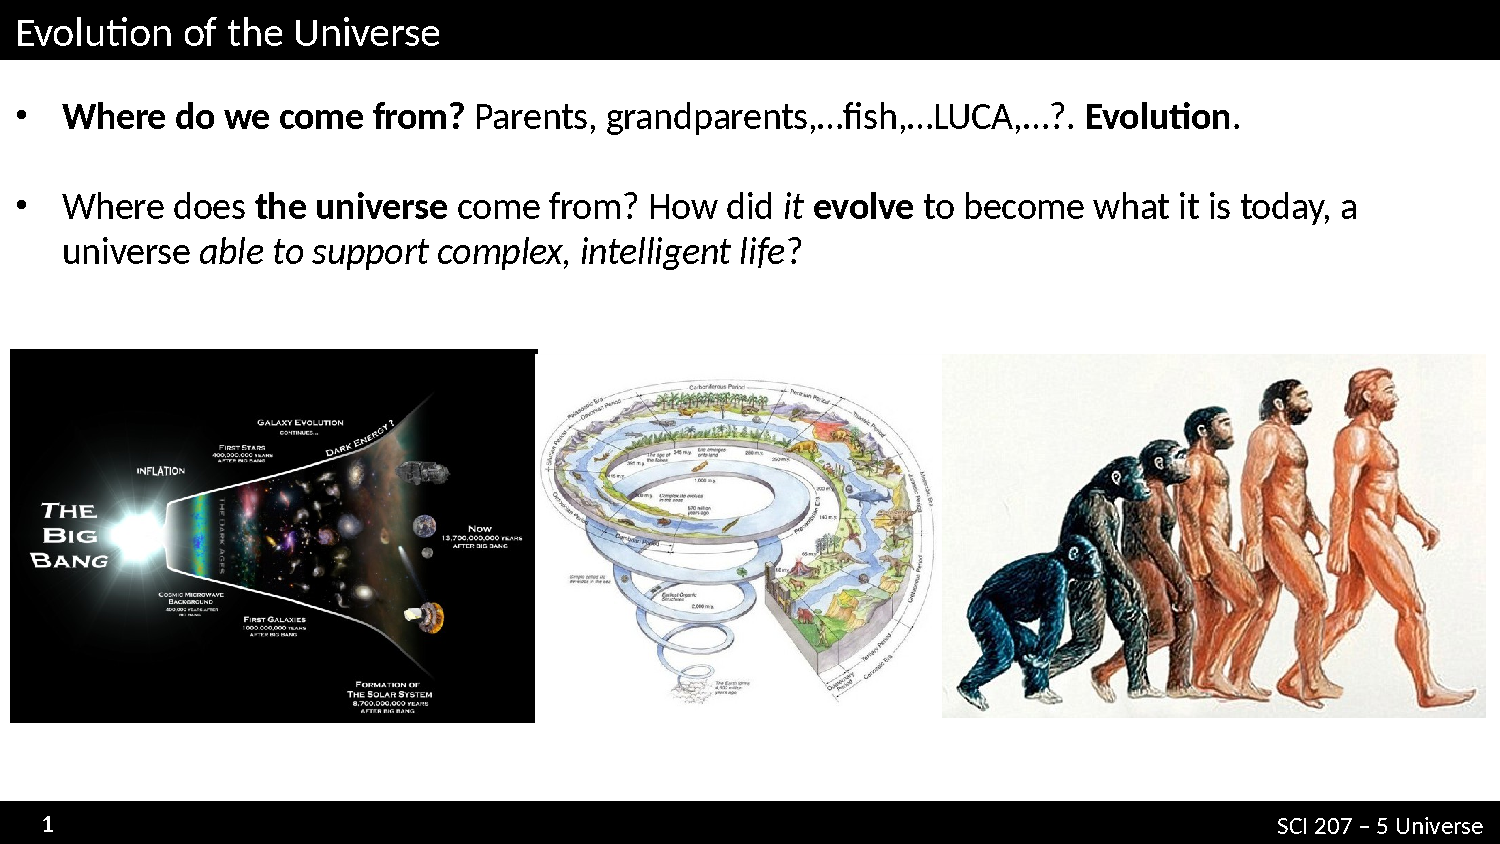
\includepdf[page=6]{slides3}
Hubble saw stars that fluctuated in brightness called Cepheids where he could calculated their true brightness based on the period of flickerings. This value combined with their apparent brightness he could calculate distances. These distances were way bigger than we thought possible which means that they were outside our galaxy and galaxies in and of themselves. This showed that not only where we in a galaxy, but the universe outside our galaxy is huge.

He also found that galaxies that are farther away are receding faster.

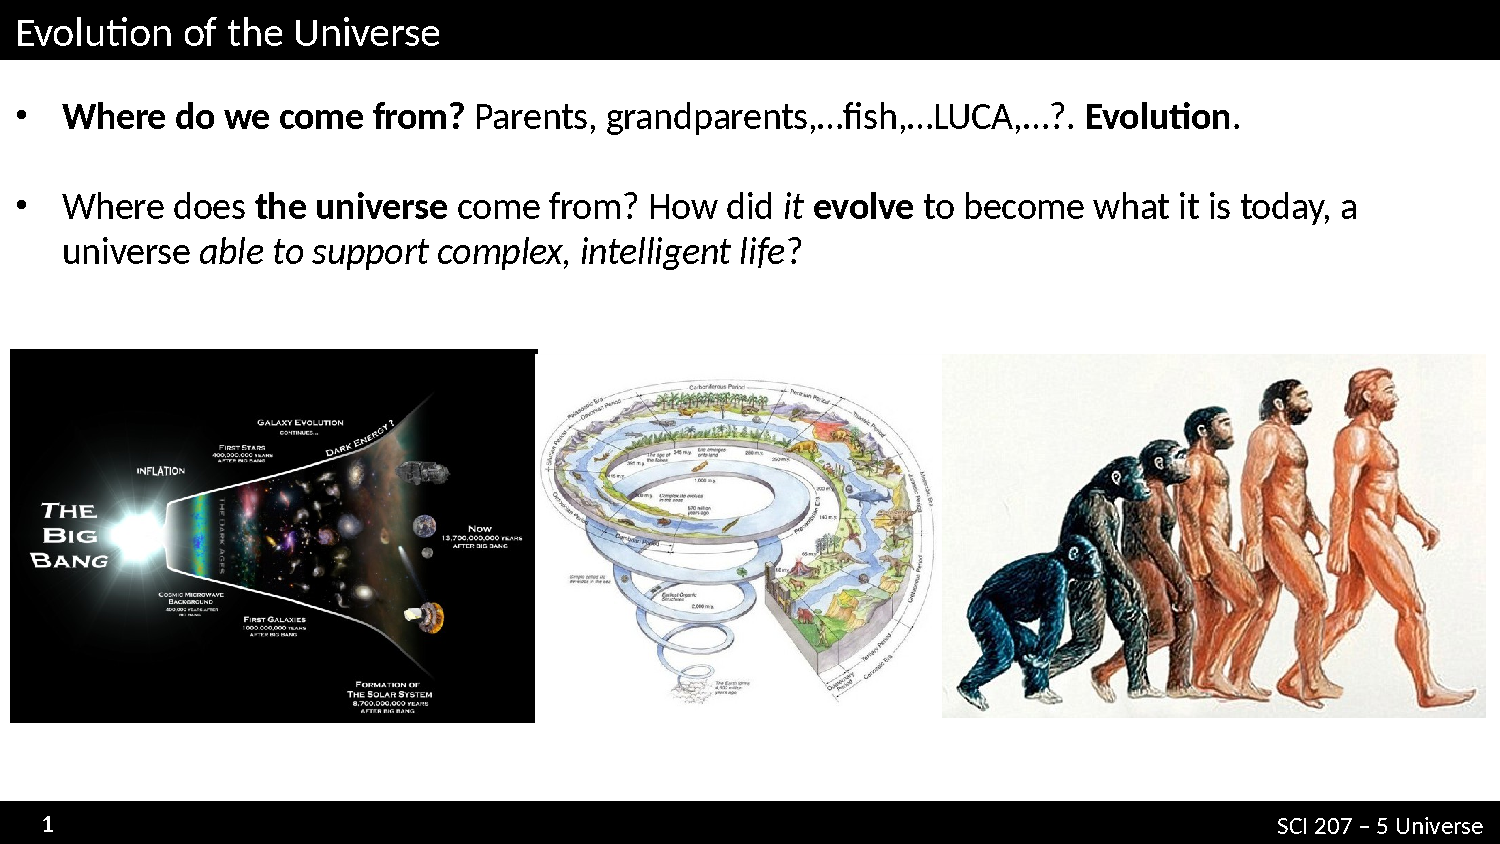
\includepdf[page=7]{slides3}
In an image of the sky the smaller dots tend to be redder (might be smaller, or just farther away).

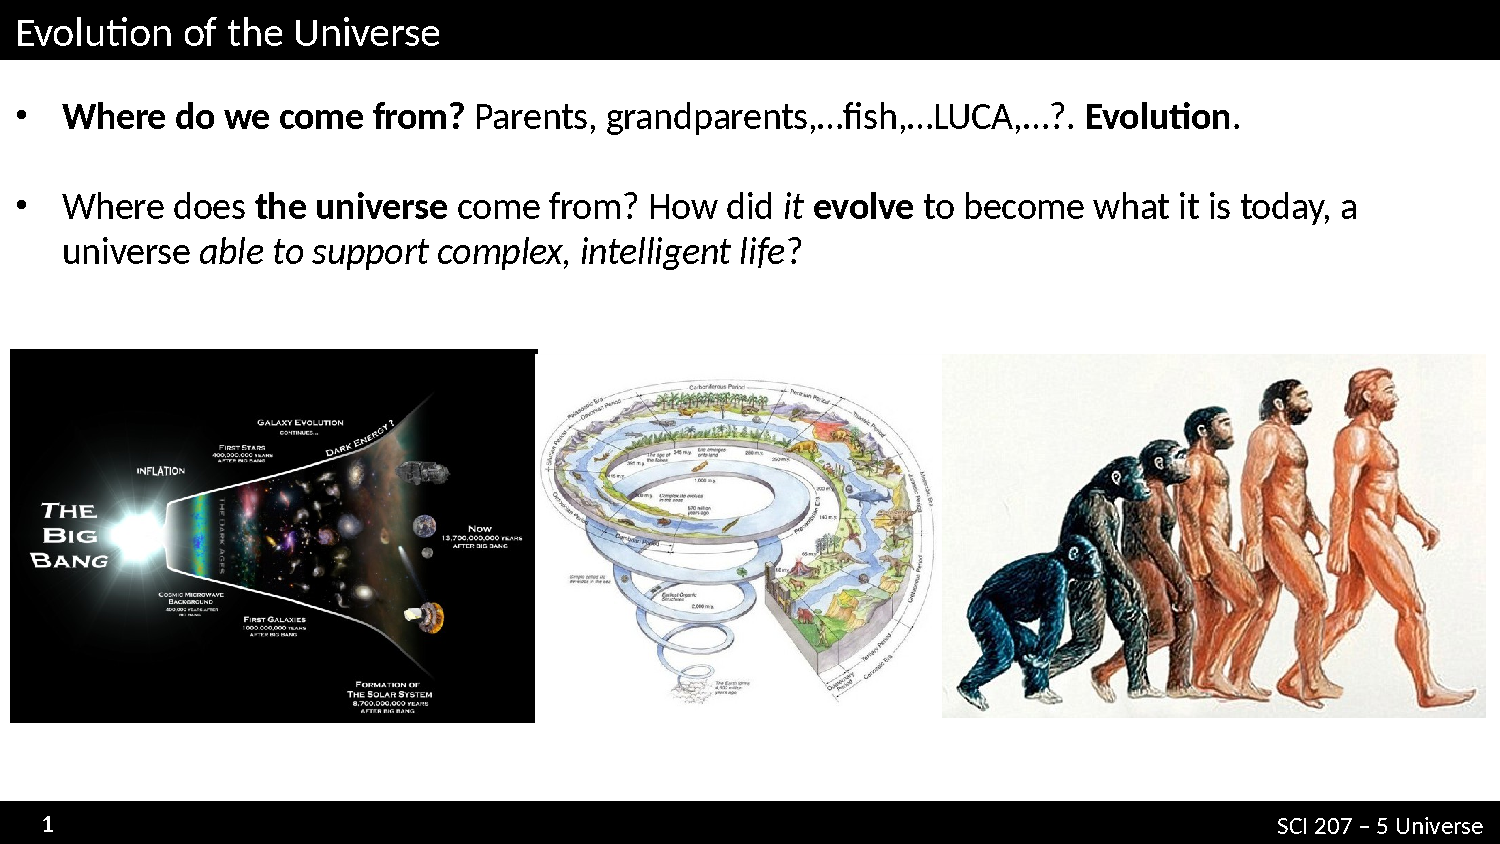
\includepdf[page=8-10]{slides3}
Hubble's law states that the apparent velocity is proportional to the distance between us. This is mainly due to the space between us expanding.

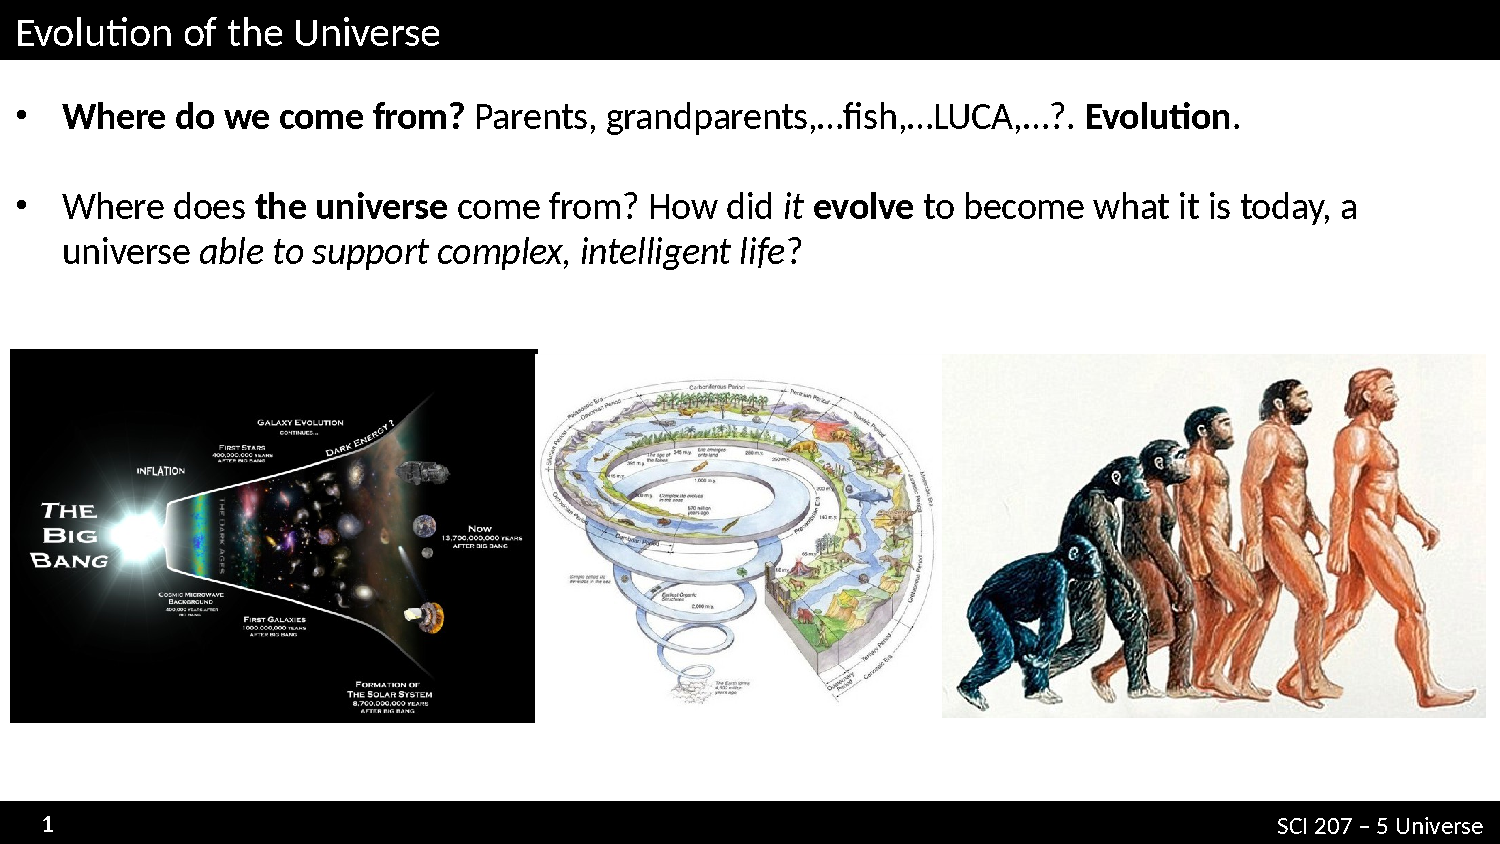
\includepdf[page=11]{slides3}
In the picture on the left, the arrow represent the velocity of galaxies. You can see that there are centers of attraction that galaxies are moving towards, these would be large clumps of dark matter. On average though the net velocity is 0.

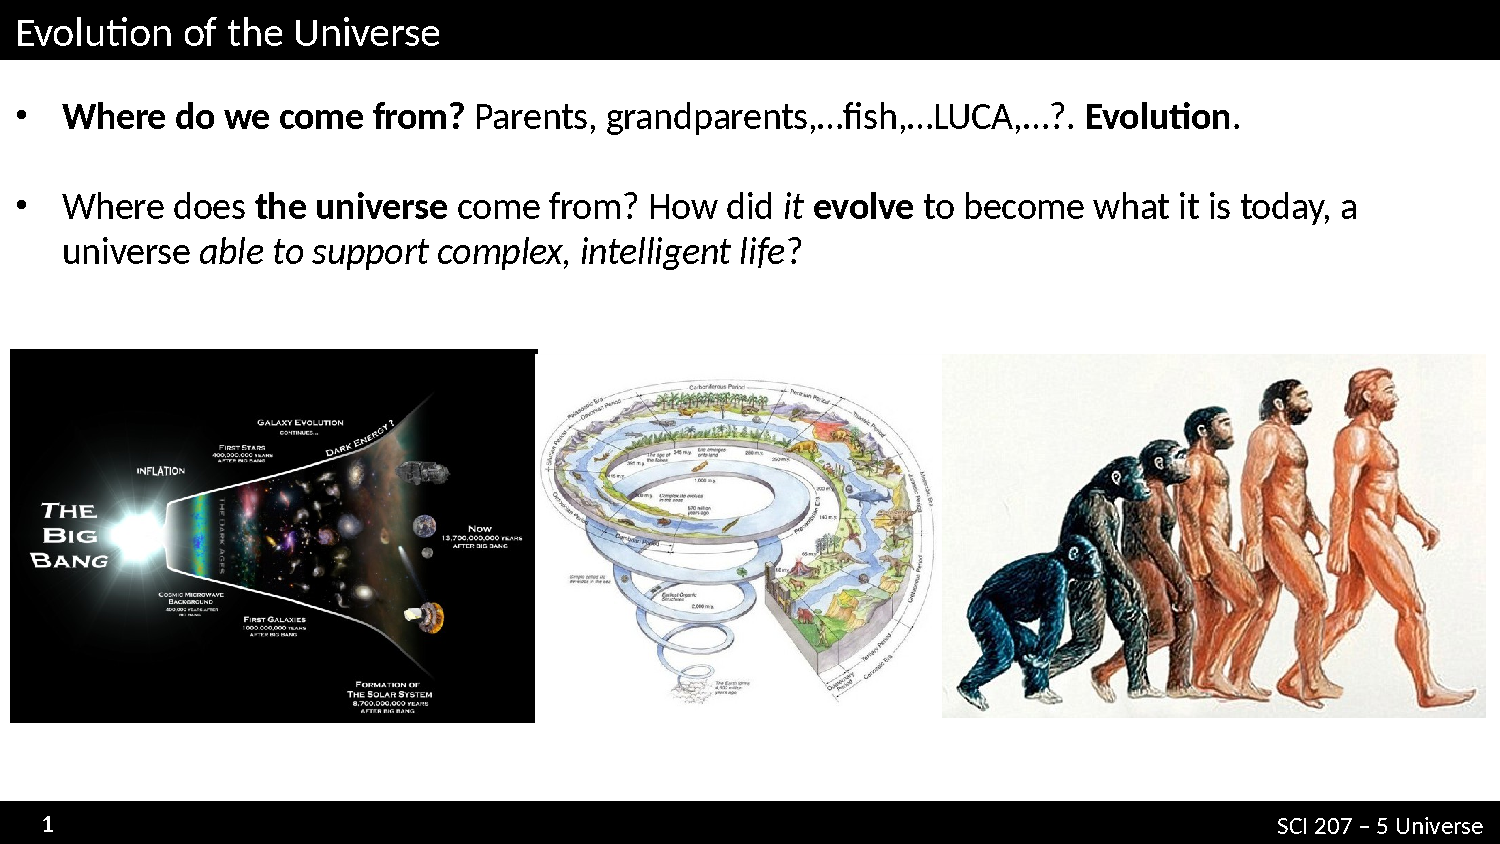
\includepdf[page=12-14]{slides3}
The galaxies dont exand, the space between them does. This explains why it appears that galaxies farther away are moving away faster.

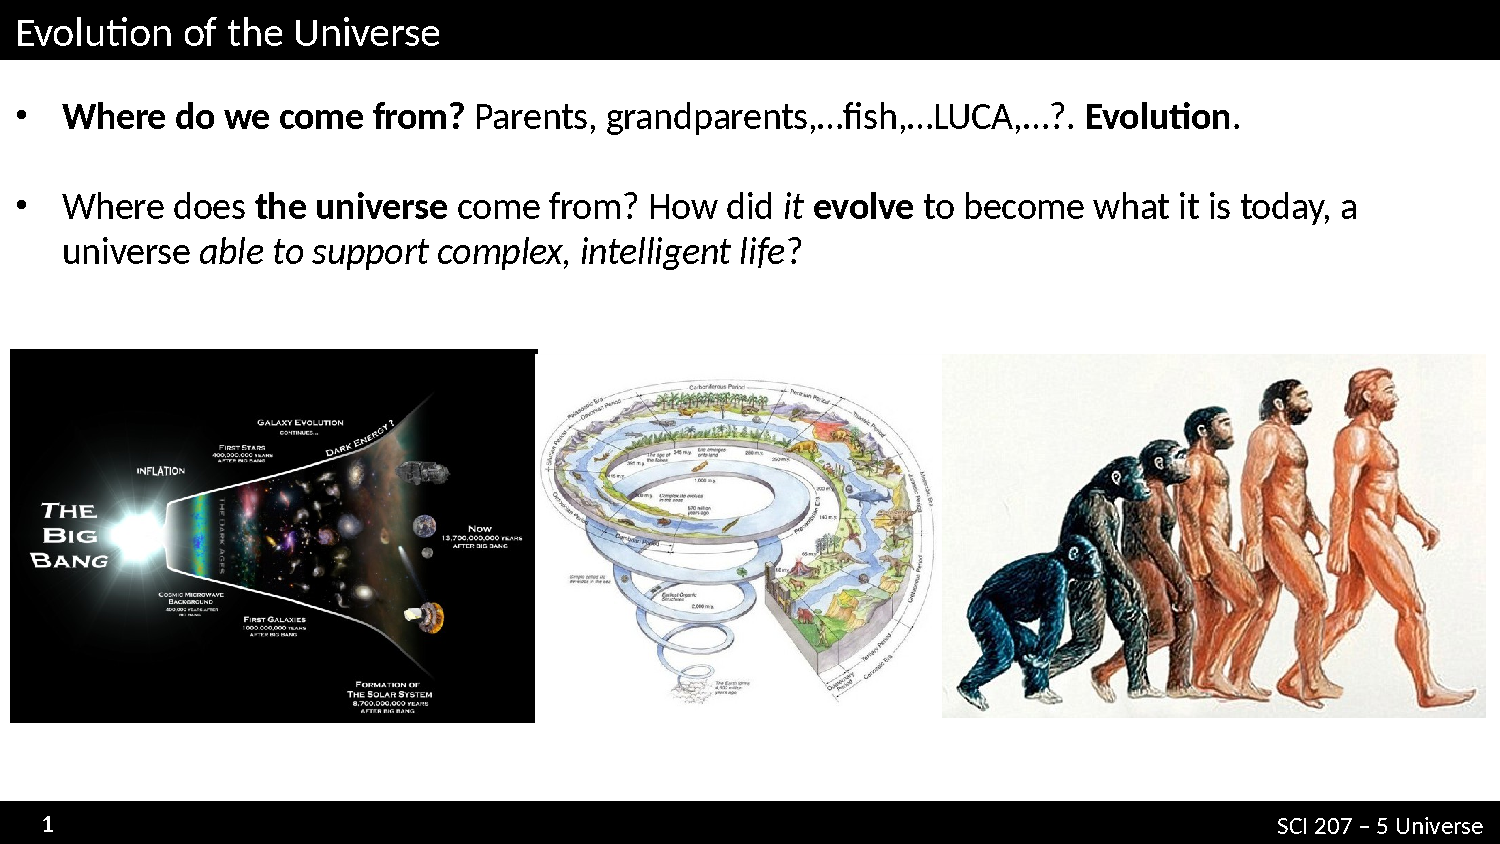
\includepdf[page=15-16]{slides3}
We can only see a small portion of space (that in our horizon).

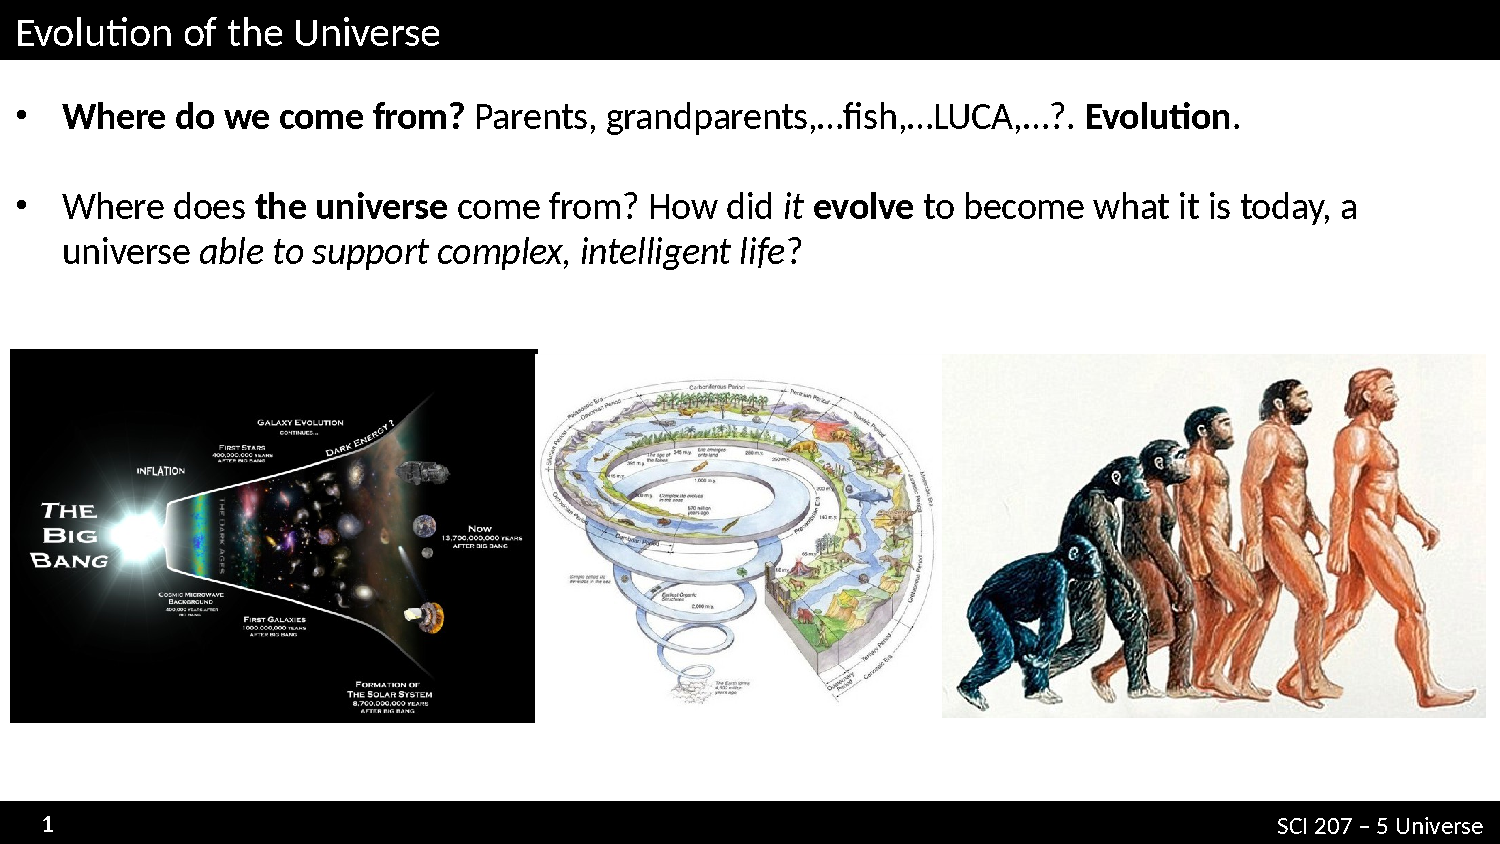
\includepdf[page=17]{slides3}
We reworded the hubble's law to derive a function for hubble's constact respective of time.

%slide 100
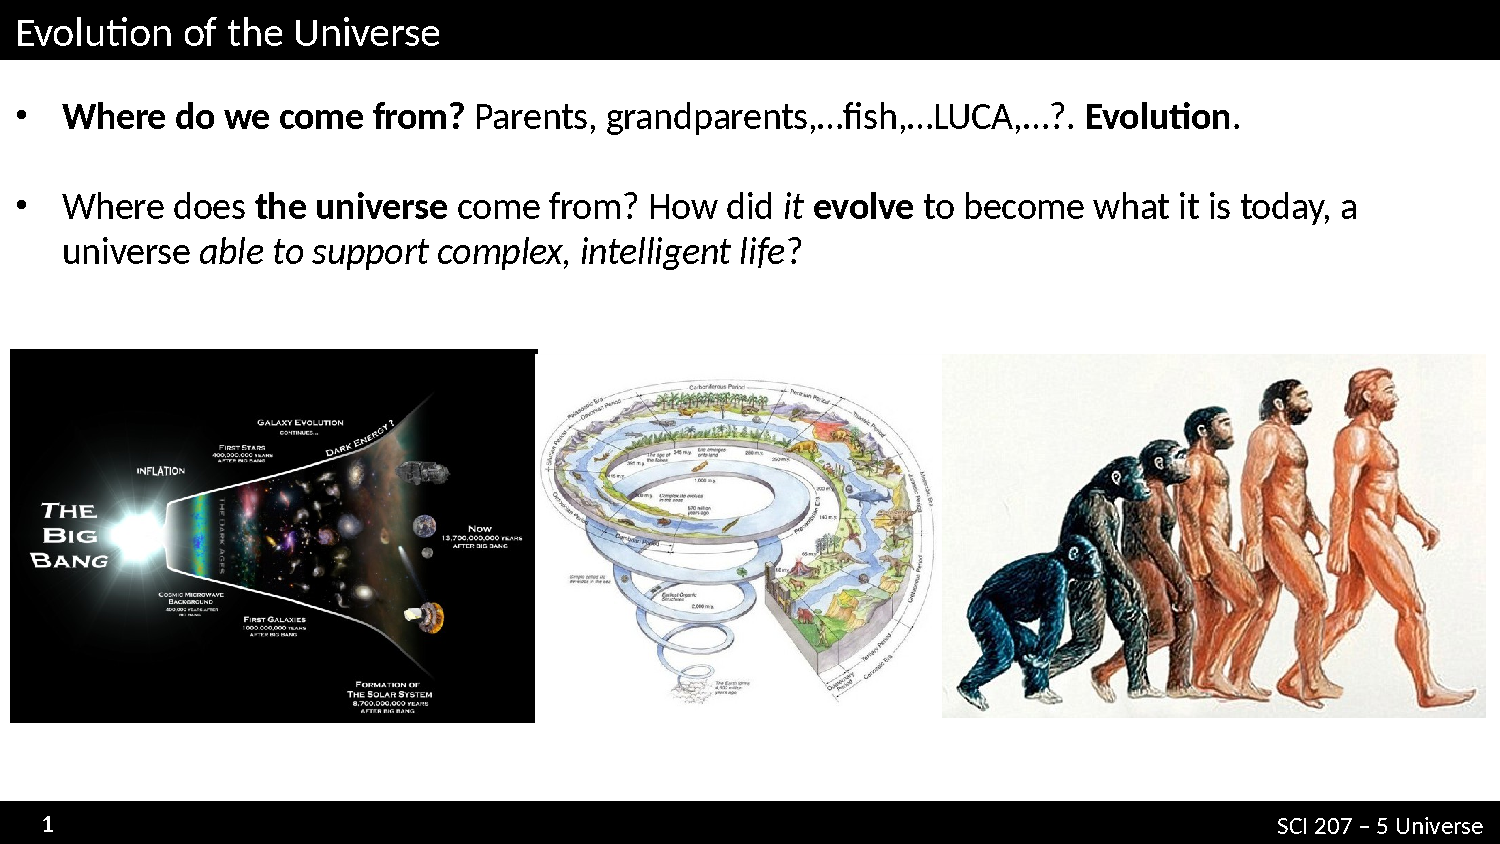
\includepdf[page=18-20]{slides3}
The universe started out uniform untill it started to expand and in doing so cooled which allowed some pockets of gravity to form. On the whole though it really is still uniform.

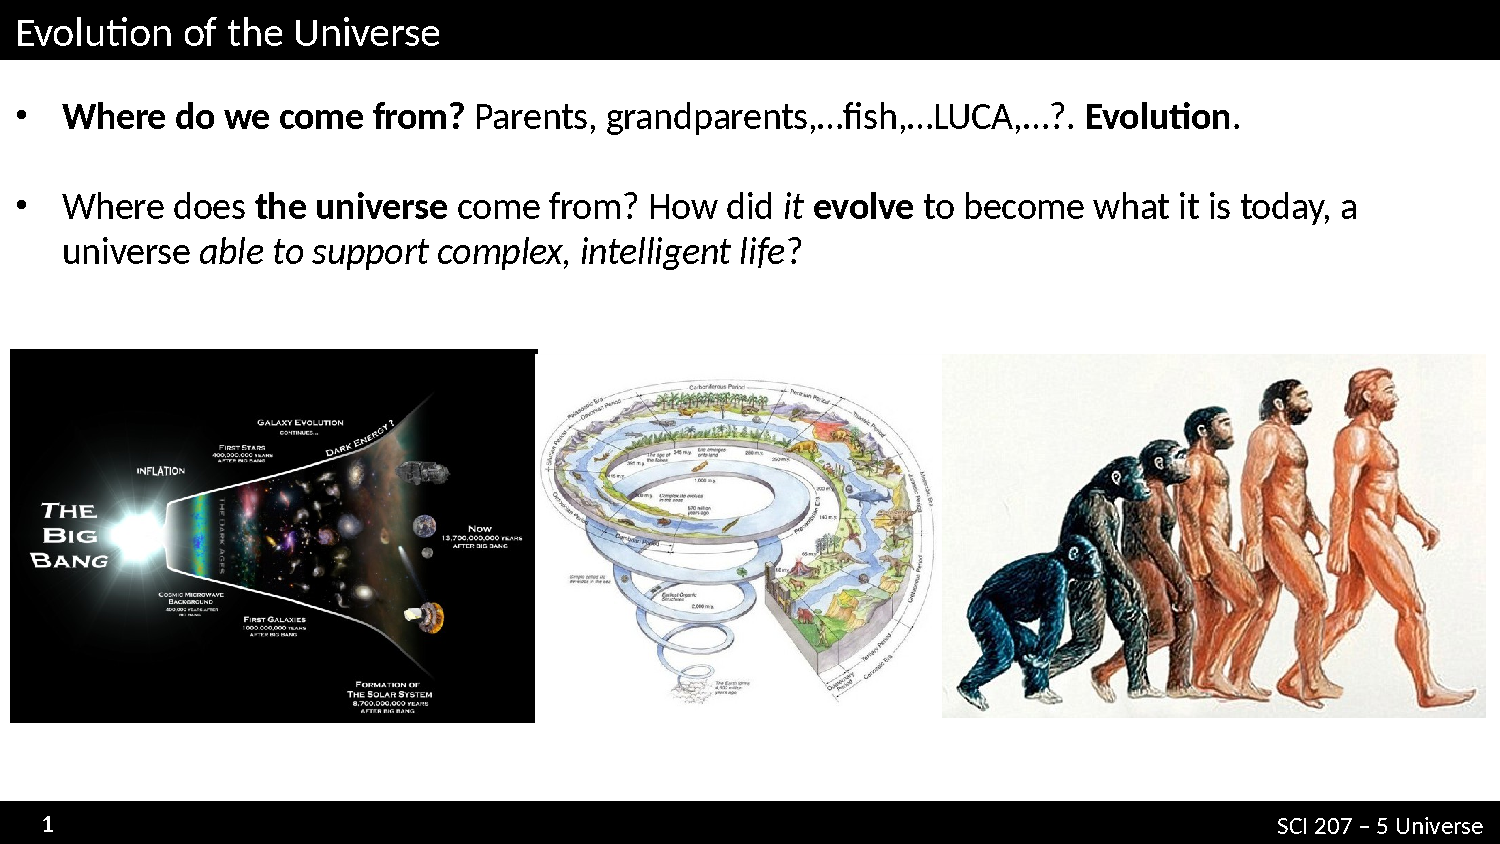
\includepdf[page=21]{slides3}
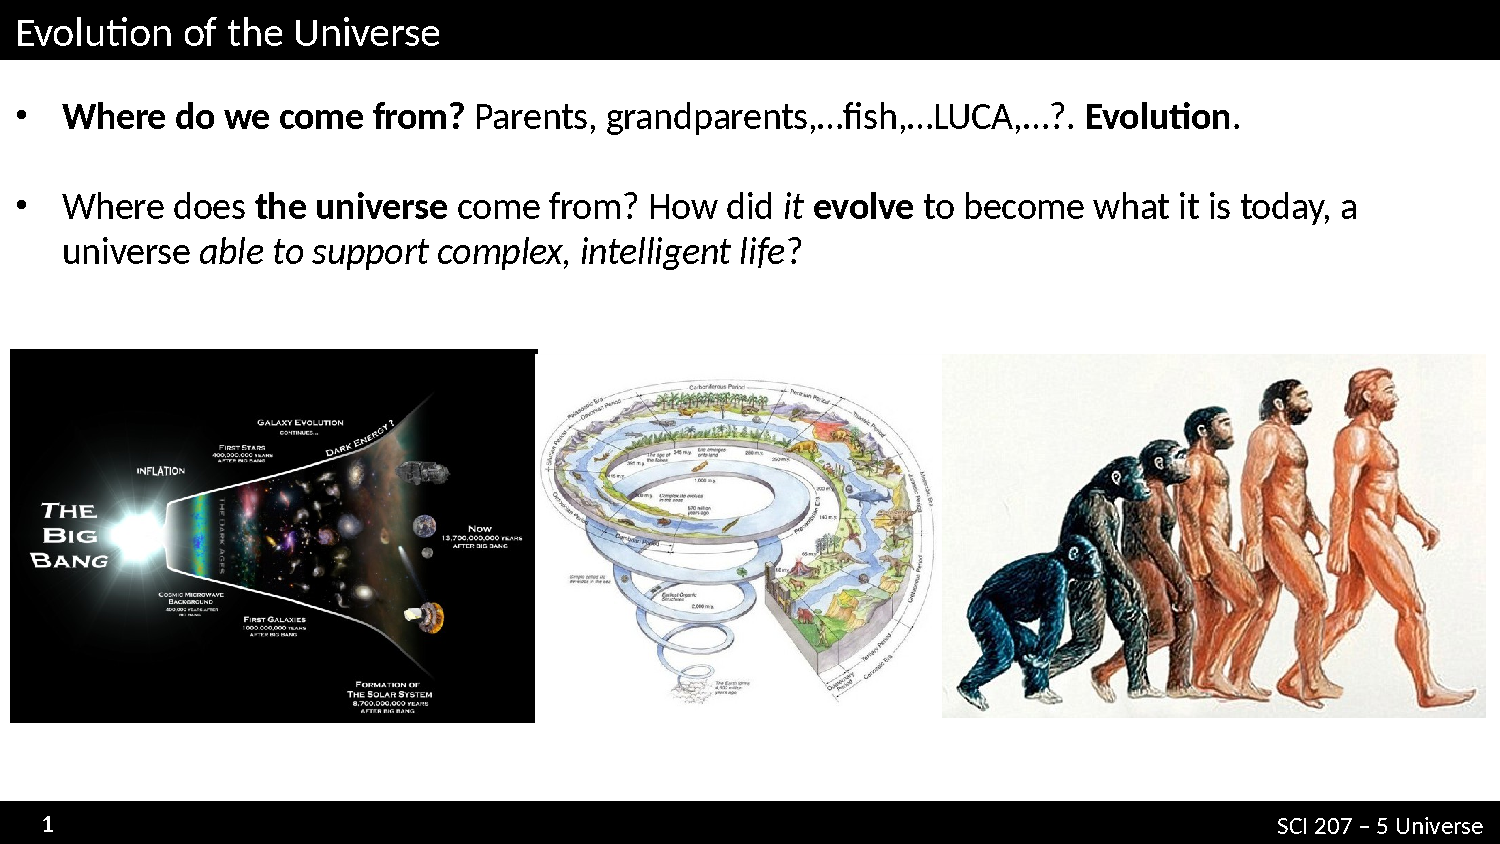
\includepdf[page=22-26]{slides3}
The dark night sky is super helpful when trying to discover if there is a start to the universe.

Lets assume the universe is static and infinitely big. If it had a physical end what is there? We dont want to consider that so we say that it is infinite. We also say that stars are evently distributed. We also say that the univere is infinitely old because we dont want to think of it as having a start.

These assumptions were held as true for a long time.111
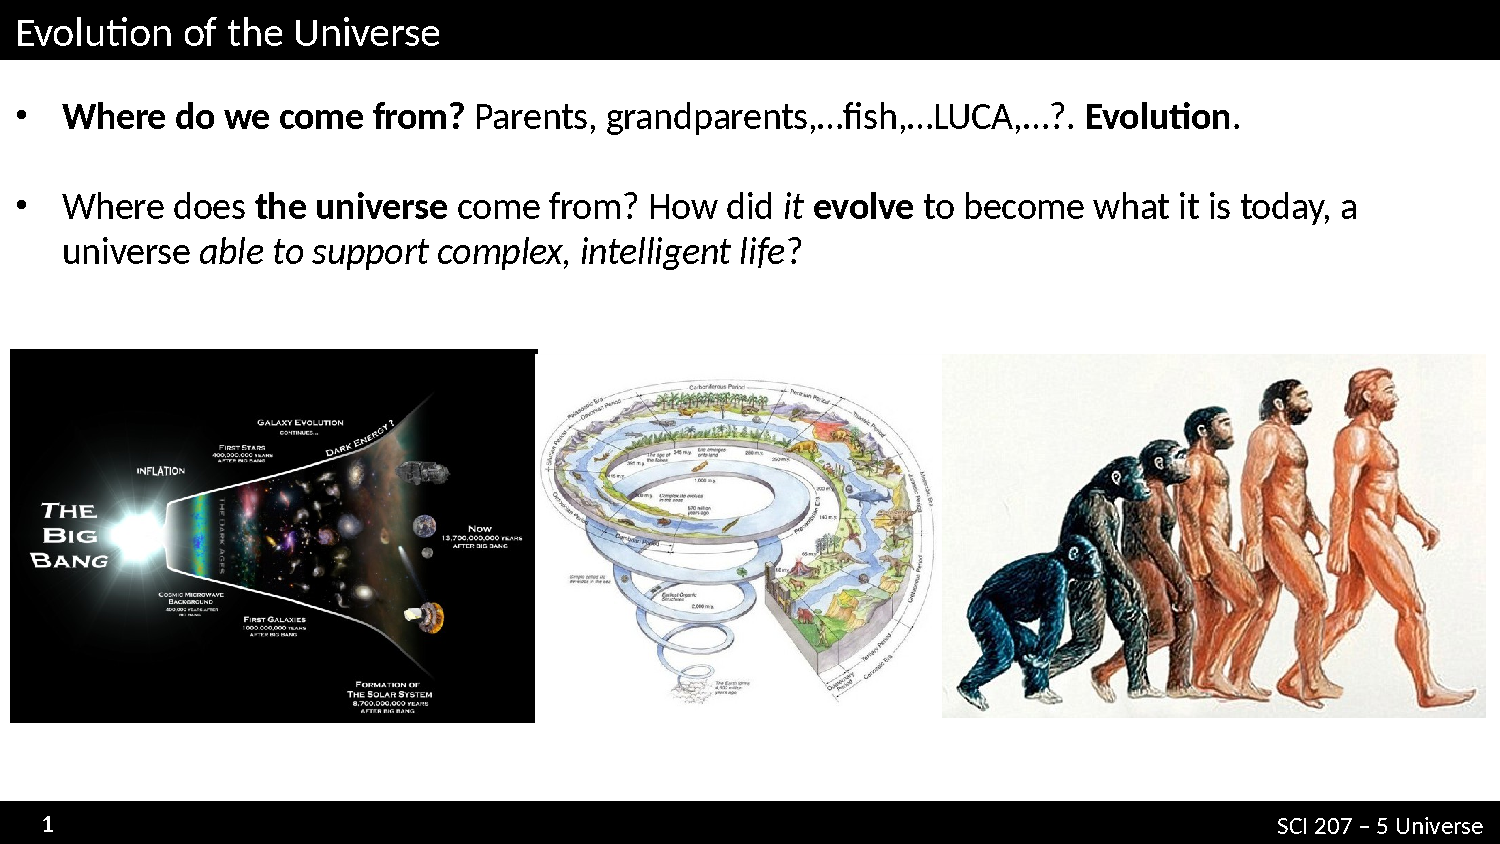
\includepdf[page=27-31]{slides3}
We should have a night sky covered in stars with no black in between. People started to get worried about this. One of their assumptions must be wrong. The infinitly big and even distribution assumptions are reasonably well accepted/proven. The universe being static is related to it being infitely old so we conclude that both of these are wrong.r

MOTHER FUCKER STOPPED PUTING PAGE NUMBERS ON HIS SLIDES, I HAVE NO CLUE WHAT SLIDE WE ARE AT NOW. SORRY FUTURE LARA, I TRIED.

We assume that the night sky has dark parts because the stars there have not had enough time to get to us. This defines the cosmological horizon as stars that are close enough for us to see. Edgar Allan Poe was the first to think of this.

welp, fuck, lots all my notes for this up to slide 207, shiiiiieeeeeettttt. should not have tried to show amanda how detached head workds without pushing first, oh well, who cares.

\paragraph{Horizon Problem}
\label{par:horizon_problem}
The temperature is almost perfectly uniform. The little blobs are almost perfectly across from each other and they are slightly different temperatures. These blobs that are on opposite sides of each other are exactly the same temperature. They are way far apart from each other so how could they communicate with each other. This needs to be explained, it is called the \textbf{Horizon Problem} since these two blobs are beyond eachother's horizon. This is solved by the idea of \textbf{Cosmic Inflation}.

\paragraph{Cosmic Inflation}
\label{par:cosmic_inflation}
Back in time, when the observable universe at our location was very small. At this time the universe was expanding incredibly rapidly. At this time all matter was exactly the same temperature. The problem with this is that the CMB should be perfectly uniform. This is not the case.

\paragraph{Space is Flat}
\label{par:space_is_flat}
We know for certain (or as certain as we can be) that the space is flat. This is a bit weird, when you think of the big bang theory. To maintain this flatness we have a very small window to work within before we collapse or warp to another form of space. This means that the universe had to be hella flat at the beginning. Scientists say this is stupidly improbably in the randomness of the big bang. Cosmic inflation also helps explain this.7 (OHHHH GOOOOODDDDD WHYYYYYYY STEEEEEEVEN???)

\paragraph{CMB is not Uniform}
\label{par:cmb_is_not_uniform}
This is very important because these small bloops of higher/lower temperature result in a slight difference in gravity. These pockets of gravity allow matter to congregate and then these snow balled into stars and planets and such. In a perfectly uniform universe this would not have happened. We think this happened because there is spontaneous creation an annihilation on a quantum level which might have caused this. The amplitude of these flucation is just right as well.

So why is there something instead of nothing?

%232
One theory is that near black holes there is a spotaneous creation of matter and antimatter pair, one part of the pair gets sucked into the black hole and the other one escapes and flys away. This particle that flys away is called hawking radiation. With inflation we are just inflating the matter and antimatter particles apart so that they cant find each other again. Where does the energy for this inflation come from.

All of the stuff in the observable universe can be created from one gram of matter using this inflation method. This is due to the massive amount of energy in the universe. This feels like we are getting something from nothing. But we could say that the negative energy of the universe and the positive energy of matter evens out to nothing. Kind of. Maybe. Not sure.

Before inflation began there was some stuff in some space, doesn't really matter what was in there. That stuff (of some amount) is suddenly super expanded. No idea what triggered this expansion currently, but people are researching it.

\paragraph{Magnetic Monopoles}
\label{par:magnetic_monopoles}
We currently have not proof that a magnet couldn't have just a north pole. A theory is that at the start of the universe it was filled with these and they influenced things. These would have gotten expanded to shit and now we can't find them.

We think there might be an inflation feild but we arent sure what it is, maybe the higgs feild. The theory also has lots of ad hoc elements where we dont really have numbers to back up some of our stuff so we take a guess and see what happens. People critisize this as things you could change to make it anything.

\paragraph{Other Origin Ideas}
\label{par:other_origin_ideas}
The \textbf{Conformal Cyclic Cosmology} theory is the idea that there is a cycle of big bangs. The \textbf{Loop Quantum Gravity} theory is that the universe started big and crunched to some finite super finite density and bounced back. We now have a deep enough understanding to try to look to what happened before the big bang. \textbf{Super String Theory} have all these crazy ideas about dimensions. There are all these extra dimensions, so our universe is a 3d surface withing this multidimensional space. An alien universe might exist somewhere else in this space and it collides with us. The energy of that motion gets turned into particles which create matter and antimatter.

\paragraph{Eternal Inflation and Multiverse}
\label{par:eternal_inflation_and_multiverse}
Lets say that the universe is infinite and eternal. We have really rapid expansions into bubbles. Throughout the universe there are bubbles of observable universes. This means that in the volume of space there are infinitely many other universes. Some might have different laws of nature.












\end{document}



